\section {Športová streľba na terč}
Streľba na terč má bohatú históriu, ktorá sa vyvinula z životne dôležitej schopnosti prežitia 
až po moderný súťažný šport. Tento vývoj bol ovplyvnený technologickým pokrokom, zmenami v 
spoločenských postojoch k strelným zbraniam a lukostreľbe a vývojom rôznych typov terčov, ako 
sú oceľové, papierové, skákacie a siluetové terče ~\cite{target_shooting}.

Streľba na terč bola zaradená do programu olympijských hier už v Paríži v roku 1896, kde sa 
prvýkrát objavila ako súťažný šport. V tomto období sa objavili rôzne formy streleckých súťaží, 
vrátane streľby na živé holuby. Po tomto ročníku bolo zavedené strieľanie na terče z umelej 
hmoty ~\cite{target_shooting_olympic}.

\subsection{Moderná streľba na terč}
Existujúce systémy na vyhodnocovanie zásahov v športovej streľbe kombinujú rôzne technológie na 
meranie a analýzu zásahov. Tieto riešenia zvyčajne zahŕňajú použitie digitálnych terčov, kamier, 
senzorov alebo iných optických zariadení, ktoré umožňujú automatické zistenie polohy zásahov na terči. 
Mnohé komerčné systémy používajú kamery na analýzu pohybu a zásahov v reálnom čase. Tieto systémy 
sú schopné poskytnúť okamžité výsledky, no sú často veľmi nákladné a vyžadujú zložité zariadenie, 
čo môže byť obmedzujúce pre amatérske alebo menšie strelecké kluby.

Niektoré z týchto riešení využívajú pokročilé metódy spracovania obrazu, ako je detekcia hrán alebo 
identifikácia štruktúr na terči, aby presne vyhodnotili zásahy. Napríklad, pri analýze obrazu sa často 
využíva technika, ktorá sleduje zmeny v pixeloch obrazu medzi jednotlivými snímkami, aby sa určilo 
miesto zásahu. V niektorých prípadoch sa využívajú algoritmy strojového učenia, ktoré sa učia rozpoznať 
vzory na terči a určiť bod zásahu s vysokou presnosťou.

Existujú aj systémy, ktoré sú zamerané na analýzu štatistík strelca počas viacerých kôl, čím umožňujú 
trénerom a športovcom lepšie pochopiť výkon a identifikovať oblasti na zlepšenie.


\section {Programovací jazyk JavaScript}
JavaScript je objektovo orientovaný, vysokoúrovňový programovací jazyk. Narozdiel od kompilovaných jazykov kde
sa najprv kód preloží do strojového kódu a následne vytvorí spustiteľný súbor ako napríklad jazyk C, C++ alebo Rust, JavaScript 
je jazyk interpretovaný - teda kód sa vykonáva riadok po riadku pomocou interpreteru.
O vznik tohoto programovacieho jazyka sa zaslúžil Brendan Eich. JavaScript bol vydaný v roku 1995 v máji a to iba za 
10 dní. Jeho prvým názvom bolo Mocha ~\cite{geeksforgeeks_js}. 
Tento programovací jazyk umožňuje implementovať komplexné funkcie na webových stránkach - zakaždým, keď webová
stránka robí viac, než len sedí a zobrazuje statické dáta - zobrazuje včasné aktualizácie obsahu, interaktívne mapy,
animovanú 2D/3D grafiku, rolovacie video jukeboxy alebo iné interaktívne prvky - ide pravdepodobne o zakomponovanie JavaScriptu ~\cite{mdn_js}. 

JavaScript patrí medzi najpoužívanejšie programovacie jazyky najmä vďaka svojej jednoduchej a flexibilnej syntaxe, ktorá umožňuje rýchly štart 
a intuitívnu prácu s webovými technológiami.

Okrem svojej úlohy pri základnej interaktivite sa JavaScript v modernej webovej architektúre presunul z doplnkového jazyka fungujúceho popri 
html a css na samotne plnohodnotný základ pre vývoj komplexných aplikácií. Vďaka vývoju frameworkov ako React, Vue či Angular sa JavaScript 
stal nástrojom nielen pre manipuláciu s DOM - Document Object Model - štruktúrovaná reprezentácia HTML, ale aj pre budovanie komponentovo 
orientovaných systémov, spracovanie stavov aplikácií, routing či prácu s API na strane klienta. Tento posun umožnil načítavanie nových bez 
opätovného načítania celej stránky. Výsledkom je rýchlejšia, plynulejšia a používateľsky prívetivejšia skúsenosť, porovnateľná s natívnymi 
aplikáciami.

\subsection{Výhody jazyka JavaScript}
Medzi veľkú výhodu jazyka patrí "Client-Side Scripting", Teda JavaScript beží v používateľovom prehliadači, to znamená, že má kratší čas 
odpovedí, pretože nie je nutné komunikovať so serverom. Veľmi kladnou záležitosťou tohoto jazyka je určite jeho všestrannosť,
JavaScript je možné použiť pre rôžnu škálu úloh, od jednoduchých výpočtov až po zložité aplikácie na strane servera. Dôvodom, prečo je jazyk tak 
populárny pri vývoji webových aplikácií je, že umožňuje reagovať na klikanie, stlačenie kláves, zmeny okna a rozhrania, atď. v reálnom čase.
Javascript funguje asynchrónne - teda zvláda úlohy ako načítanie dát zo servera bez toho aby zamrzlo používaťeľské rozhranie. Vďaka 
obľúbenosti tohoto jazyka medzi  programátormi po celom svete, tento jazyk disponuje množstvom dokumentácie a tutoriálov ~\cite{gfg_intro_js}.

\subsection{Nevýhody jazyka JavaScript}
JavaScript je interpretovaný jazyk, to znamená, že je pomalší ako kompilované jazyky ako sú C, C++ alebo Pascal. 
Keďže JavaScript beží na strane klienta, je náchylný na útoky ako Cross-Site Scripting (XSS) a Cross-Site Request Forgery (CSRF).
JavaScript je dynamicky typovaný jazyk, čo znamená, že typy premenných nie sú striktne definované. To môže viesť k chybám, ktoré sa 
objavia až pri spustení programu, a sťažuje to údržbu väčších kódových báz. JavaScript sa vo veľkej miere spolieha na asynchrónne programovanie, 
čo môže byť pre vývojárov náročné na pochopenie a správne implementovanie. Aj keď moderné konštrukcie ako Promises a async/await pomáhajú, 
stále existuje riziko vzniku tzv. "callback hell" ~\cite{itpedia_js_downsides}.


\section{PWA}
PWA je skratkou pre progressive web app - teda progresívna webová aplikácia. 


\section{OpenCV}
OpenCV je skratka pre Open Source Computer Vision a je to knižnica funkcií, ktoré sú užitočné pri programovaní 
aplikácií počítačového videnia v reálnom čase. Termín počítačové videnie sa používa pre subjekt, ktorý vykonáva 
analýzu digitálnych obrázkov a videí pomocou počítačového programu. Počítačové videnie je dôležitou súčasťou 
moderných disciplín, akými sú umelá inteligencia a strojové učenie ~\cite{tutorialspoint_opencv}. V práci 
spomínam funkcie mnou považované za kľúčové pre túto prácu, samotná knižnica disponuje nikoľkonásobne viac 
funkciami, pre viac informácií je dostupná dokumentácia knižnice ~\cite{documentation_opencv}.

\subsection{Čítanie obrázkov}
Medzi jednu z najdôležitejších funckcií knižnice patrí funkcia na čítanie obrázkov. Knižnica OpenCV poskytuje 
funkciu s názvom imread(), ktorá slúži na načítanie obrázku do pamäte zo zvoleného súboru pomocou prvého argumentu 
funkcie.  

Funkcia prečíta obrázok a uloží ho vo formáte matice, kde tvar matice zodpovedá rozmerom obrázka. Druhým argumentom 
funkcie je parameter menom flags. Tento parameter rozhoduje o tom ako je obrázok načítaný, teda môže byť načítaný 
ako farebný (predvolené), šedý (jeden kanál) alebo nezmenený, teda čítaný taký aký je, ale zachovávajúci všetky 
kanály transparentnosti.

\subsection{Vlastnosti obrázka}
Medzi funkcie pracujúce s vlastnosťami obrázkov radíme funkcie shape() a resize()

Funkcia shape() sa používa na získanie rozmerov obrázka alebo matrice. Táto funkcia vráti veľkosť obrázka alebo 
matice ako n-ticu, čo môže byť užitočné na pochopenie štruktúry údajov. Často sa používa na kontrolu vlastností 
obrazu, ako sú šírka, výška a farebné kanály.

Funkcia resize() sa používa na zmenu veľkosti obrázka na zadanú veľkosť alebo podľa danej mierky. Táto funkcia 
je kľúčová pri mnohých úlohách spracovania obrazu, kde je potrebné upraviť veľkosť obrázkov pred vykonaním operácií, 
ako je detekcia alebo klasifikácia objektov.

\subsection{Vyobrazenie geometrických útvarov}
Kreslenie tvarov a textu na obrázky je užitočné na vizualizáciu údajov alebo anotácií v aplikáciách počítačového 
videnia. OpenCV poskytuje rôzne funkcie na kreslenie základných tvarov ako sú čiary(cv2.line), obdĺžniky(cv2.rectangle) 
a kruhy(cv2.circle), taktiež umožňuje pridávanie textu(cv2.puText) do obrázkov.

%%%%%%%%%%%%%%%%%%%%%%%%%%%%%%%%
%%                            %%
%% Štruktúra záverečnej práce %%
%%                            %%
%%%%%%%%%%%%%%%%%%%%%%%%%%%%%%%%
\section{Štruktúra záverečnej práce}\label{sec:StrukturaPrace}
Za záverečnú prácu považujeme bakalársku, diplomovú
a~dizertačnú prácu \cite{zakon1312002}.
Práca napísaná v~slovenskom jazyku má tieto časti \cite{vyhlaska2332011, usmernenie562011}:
\begin{enumerate}
    \item Úvodná časť
    \begin{enumerate}
        \item obal
        \item titulný list
        \item zadanie
        \item poďakovanie (nepovinné)
        \item abstrakt v slovenskom jazyku
        \item abstrakt v anglickom jazyku
        \item obsah
        \item zoznam ilustrácií, obrázkov (nepovinné)
        \item zoznam tabuliek (nepovinné)
        \item zoznam skratiek a značiek (odporúčané)
    \end{enumerate}
    \item Hlavná textová časť
    \begin{enumerate}
        \item úvod
        \item jadro
        \begin{itemize}
            \item súčasný stav riešenej problematiky doma a v zahraničí
            \item cieľ práce
            \item metodika práce a metódy skúmania
            \item výsledky práce
            \item diskusia
        \end{itemize}
        \item záver
        \item zoznam použitej literatúry
    \end{enumerate}
    \item Záverečná časť
    \begin{enumerate}
        \item dodatky (podľa potreby)
        \item prílohy (podľa potreby)
    \end{enumerate}
\end{enumerate}

\subsection{Úvodná časť práce}
Hlavným obsahom úvodnej časti sú formálne náležitosti práce a musia byť zaradené v~poradí podľa zoznamu v~úvode tejto kapitoly.

\subsubsection{Obálka, titulný list, zadanie}
Začiatočné stránky práce automaticky generuje univerzitný
informačný systém AIS vo formáte PDF.
Môžeme ich do záverečnej práce vložiť pomocou príkazu \verb|\includepdf| z~balíčka \verb|pdfpages|
alebo využijeme makrá \verb|FEIcover| a~\verb|FEItitle| na vytvorenie obálky a prvej
stránky práce.
Aby boli všetky informácie aktuálne,
treba venovať pozornosť vyplneniu údajových
premenných v~úvode hlavného súboru \verb|thesis.tex|.

Zadanie odporúčame vložiť pomocou spomínaného makra
\verb|\includepdf| tak, že najprv uložíme PDF súbor
so zadaním do priečinka \verb|includes| a prepíšeme
názov súboru v argumente makra.

\subsubsection{Poďakovanie}
Nepovinná, ale veľmi obľúbená časť práce.
Je umiestnené na samostatnej strane zväčša v~dolnej časti.
Jej obsah je ponechaný na autora.
Obsah poďakovania sa nachádza v~súbore
\verb|includes/thanks.tex| a~sadzbu má na starosti
príkaz \verb|\FEIthanks|.

\subsubsection{Slovenský a anglický abstrakt}
Definícia abstraktu vychádza z technickej normy STN ISO 214 Dokumentácia.
Abstrakty (referáty) pre publikácie a dokumentáciu \cite{iso214}.
Termín abstrakt je skrátené, presné vyjadrenie obsahu
bez pridanej interpretácie a kritiky.
Mal by poskytovať čo najviac informácií obsiahnutých v~dokumente.

Abstrakt si netreba zamieňať s termínmi anotácia,
extrakt alebo rezumé.
Anotácia je stručná poznámka, alebo vysvetlenie,
prípadne veľmi stručný opis dokumentu alebo jeho obsahu.
Extrakt predstavuje časti dokumentu vybratých
na reprezentáciu celku.
Rezumé obsahuje stručné zopakovanie významných prínosov
a~záverov v práci.
Nachádza sa zvyčajne na konci dokumentu
a~slúži na doplnenie orientácie čitateľa,
ktorý študoval predchádzajúci text.
Ak je práca napísaná v~anglickom jazyku,
musí obsahovať rezumé v~slovenčine.
V~slovenskej práci nemusí byť rezumé.

\paragraph{Účel a použitie abstraktov}
\begin{itemize}\it
  \item \uv{Dobre vypracovaný abstrakt umožní čitateľom identifikovať
  základný obsah dokumentu, rýchlo a presne stanoviť jeho
  relevanciu, a tak sa rozhodnúť, či potrebujú čítať celý
  dokument.}

  \item \uv{Čitatelia, pre ktorých predstavuje dokument len okrajový
  záujem, často získajú z~abstraktu dostatok informácií a nemusia
  čítať celý dokument.}

  \item \uv{Abstrakty sú často cenné aj pri automatickom vyhľadávaní
  v~plných textoch na získanie predbežných informácií a na
  informačný prieskum.}
\end{itemize}
\begin{flushright}
(Citované z normy STN ISO 214 \cite{iso214})
\end{flushright}

Podľa metodického usmernenia Ministerstva školstva, vedy, výskumu a športu SR č. 56/2011 (čl. 1, ods. 1)
\emph{\uv{abstrakt obsahuje informáciu o cieľoch práce,
jej stručnom obsahu a~v~závere abstraktu
sa charakterizuje splnenie cieľa,
výsledky a~význam celej práce.
Súčasťou abstraktu je 3 -- 5 kľúčových slov.
Abstrakt sa píše súvisle ako jeden odsek a jeho rozsah je
spravidla 100 až 500 slov}}~\cite{usmernenie562011}.

Text slovenského a~anglického abstraktu sa nachádzajú
v~súboroch \verb|attachment.tex| a~\verb|attachmentEN.tex| v~priečinku \verb|includes|.

Do dokumentu ich vložia makrá šablóny
\verb|\FEIabstract| a~\verb|\FEIabstractEN|
v~hlavnom súbore \verb|thesis.tex|.
Každé makro má jeden povinný parameter --
cesta a~názov súboru s~textom abstraktu.
Makrá zároveň vytlačia pod abstrakty
v každom jazyku zoznam kľúčových slov.

\subsubsection{Obsah a zoznamy}
Obsah je povinný prehľad jednotlivých kapitol
a~častí práce s~uvedením nadpisov a~strán.
Začína na samostatnej stránke ako nová kapitola
s~nadpisom Obsah bez číslovania,
ktorý sa ale v~samotnom prehľade kapitol nezobrazí.

V~\LaTeX-u zabezpečuje generovanie obsahu príkaz \verb|\tableofcontents|,
ktorý v~mieste použitia vloží automatický zoznam kapitol s~číslami strán.
Obsah vytvára na základe použitia nadpisov \verb|\section|,
\verb|\subsection| a \verb|\subsubsection|.
Toto makro vytvorí v~pracovnom adresári pomocný textový súbor
s~príponou .toc a~na základe neho generuje finálnu podobu obsahu.
Z~toho dôvodu je potrebné kompilátor \LaTeX-u
spustiť minimálne dvakrát za sebou.

V tejto šablóne má na starosti vytvorenie obsahu makro \verb|\FEIcontent|.

\subsubsection*{\normalsize Zoznam ilustrácií,
obrázkov a tabuliek}
Sú to nepovinné prehľady tzv. plávajúcich objektov.
\LaTeX\ pozná na tento účel dva príkazy: \verb|\listoffigures| a~\verb|\listoftables|. Šablóna FEIstyle ponúka alternatívne makrá \verb|\FEIlistOfFigures| a~\verb|\FEIlistOfTables|, ktoré okrem toho nastavia požadovaný typ stránky bez číslovania.

Zvlášť užitočný je príkaz \verb|\FEIlistOfFiguresAndTables|.
Vytvorí totiž spojený zoznam obrázkov a tabuliek s jedným nadpisom.

Ak zoznamy v práci nechceme, môžeme príslušné príkazy z~hlavného súboru \verb|thesis.tex| vymazať alebo ich označiť ako komentár.

\subsubsection*{\normalsize Zoznam skratiek a značiek}
V textových výstupoch vedecko-technických odborov sa používa
množstvo značiek a~skratiek najmä na označenie fyzikálnych
veličín v matematických vzťahoch,
ale aj zostručnenie textového prejavu najmä pri zložitých názvoch
vedeckých metód, zariadení alebo javov.
Sú to napríklad RTG (röntgenové žiarenie),
AFM (mikroskop atómových síl),
TEM (transmisný elektrónový mikroskop),
IR (infračervené žiarenie),
AC (obvod striedavého prúdu) a~mnoho iných.
Ak sa v práci objavia, musí ich autor pri ich prvom výskyte
jasne zadefinovať,
prípadne vysvetliť anglický preklad.
Rovnako to platí pre všetky použité fyzikálne veličiny.

Aj keď je tento zoznam nepovinná súčasť práce,
odporúčame ho zaradiť kvôli lepšej orientácii čitateľa.
Zoznam má podobu slovníka,
značky uvádzame v~abecednom poradí.

Šablóna ponúka dva spôsoby vytvorenia zoznamu a~práce so skratkami a~značkami v~texte.
\begin{enumerate}
\item Použitie nástrojov balíka \verb|glossary| umožňuje plne automatickú kontrolu nad veľkým množstvom skratiek. Skratky treba najprv definovať v externom súbore \verb|glossary.tex| a~potom ich môžeme v práci používať dvomi spôsobmi. Pri prvom výskyte použijeme skratku aj s~jej opisom, čo zariadi príkaz \verb|acrfull|.
Pri ďalších výskytoch v texte už stačí používať iba skrátený tvar pomocou príkazu \verb|acrshort|.

Po prvom skompilovaní je potrebné spustiť externý program \verb|makeglossaries| a~text skompilovať znova, prípadne kvôli správnemu radeniu strán v~obsahu, treba kompiláciu spustiť aj tretíkrát.
Podobná procedúra sa vyžaduje aj pri práci s~citáciami v systéme Bib\LaTeX.
Makro \verb|\FEIlistOfGlossaries| vytvorí abecedne zoradený zoznam.

Ak sa rozhodneme pre túto možnosť,
treba v hlavnom súbore \verb|thesis.tex| odstrániť
znak komentára pred príkazmi
\verb|\FEIglossaries{includes/glossary}|
a~\verb|\FEIlistOfGlossaries|. Pozor, tieto dva
riadky sa v súbore \verb|thesis.tex|
nachádzajú na rôznych miestach.
Nepremiestňujeme ich.

Balík \verb|glossaries| je nesporne praktická pomôcka, plnohodnotne však funguje iba v anglickom jazyku.
Pri jeho používaní narazíme na problém so skratkami, ktoré pochádzajú z anglických slov.
V slovenskom texte však musíme používať ich terminologické ekvivalenty.
Aj keď si nakoniec vytvoríme slovenský zoznam skratiek, ich automatické použitie bude limitované pri skloňovaní alebo časovaní jednotlivých výrazov.

Viac sa o možnostiach balíka dozvieme z tutoriálu na stránke \href{https://www.ctan.org/pkg/glossaries}{\texttt{www.ctan.org/pkg/ glossaries}}

\item Skratky zadáme manuálne.
Automatické riešenie v predchádzajúcom bode úplne zlyháva pri práci s veličinami, ktorých zoznam predstavuje praktickú pomôcku najmä vo fyzikálnych a~matematických oblastiach techniky. Na označovanie veličín používame rôzne symboly a ich modifikácie, napríklad písmená gréckej abecedy ($\alpha, \omega, \xi$), symboly so šípkami v prípade vektorov ($\vec r, \vec\varphi, \vec\imath$), preškrtnuté h ($\hbar$), zdvojené symboly ako $\mathbb Z$, prípadne aj niečo takéto: $\aleph_0$, čo je hebrejské písmeno alef.

Súbor \verb|manual_glossary.tex| obsahuje príklad, ako by mohol takýto ručne vyrobený zoznam vyzerať.
Makro
\verb|\FEImanualListOfGlossaries|, ktorého parameter je cesta a názov spomínaného súboru, zariadi samotnú sadzbu.
Zoznam si môžeme postupne vytvárať pri písaní a~udržiavať ho v abecednom poradí.
\end{enumerate}

\subsubsection*{\normalsize Zoznamy algoritmov a výpisov kódov programov}
Tieto typy zoznamov vytvoria makrá \verb|\FEIlistOfAlgorithms|, \verb|\FEIlistOfListings| a~sú špecifické pre informatické odbory.

Ak v práci nemáme výpisy kódov alebo algoritmy,
bude potrebné riadky s týmito príkazmi vymazať alebo označiť ako komentár. O~uvádzaní častí kódov
a~zápisov algoritmov píšeme v kapitole \ref{sec:listings}.

\subsection{Hlavná textová časť}
Samotný autorský obsah práce začína až tu.
Tradične text členíme na úvod, jadro a~záver,
pričom úvod a~záver sú samostatné kapitoly,
ktoré nečíslujeme a~je vhodné,
ak ich označíme nadpismi \emph{Úvod} a~\emph{Záver}.
Strednú časť -- jadro -- neoznačujeme.

\subsubsection{Úvod}
Prvá kapitola hlavnej časti práce má názov úvod, nečíslujeme ju.
Ide o~ucelený text v~rozsahu niekoľkých súvislých odsekov textu,
v~ktorých stručne a~výstižne charakterizujeme stav poznania
a~praxe v~danej oblasti,
oboznámime čitateľa s~cieľmi a~závermi práce.
Nosnou myšlienkou úvodu okrem uvedenia čitateľa do problematiky
je jasná motivácia autora a~jeho postoje,
ktoré viedli k~spracovaniu témy práce [3].

Nepísané pravidlo hovorí,
že úvod a~záver práce sa píšu až ako posledné.
Tento poznatok vyplýva z~praxe a~má dva dôvody:
1.~na začiatku nemusí byť úplne zrejmé, čo všetko sa v~práci naozaj objaví;
2.~úvod predstavuje samostatnú literárnu formu,
na ktorej sa neskúsený autor zasekne už na začiatku.
Aby sme sa tomu vyhli,
necháme si jeho napísanie až na záver,
keď už bude väčšina hlavného obsahu práce hotová.

Text úvodu sa nachádza v súbore \verb|includes/introduction.tex|
a~jeho sadzbu zariadi makro \verb|\FEIintroduction{includes/introduction}|.

\subsubsection{Jadro}
Táto časť práce \emph{nezačína} nadpisom \emph{Jadro}.
Obsah jadra členíme zvyčajne na niekoľko číslovaných
kapitol počínajúc číslom 1.
Prvá kapitola býva prehľad súčasného stavu problematiky,
ale môže mať aj iný názov,
napríklad \emph{Teoretická časť,} alebo rovno názov oblasti,
o~ktorej sa v nej bude písať
(trebárs \emph{Metóda prenosových matíc}).

Pri písaní strednej časti práce nemusíme postupovať úplne
striktne podľa tohto návodu.
Treba však pamätať na to,
aby sme jasne oddelili poznatky,
ktoré pochádzajú od iných autorov,
a~sú súčasťou všeobecného prehľadu,
od poznatkov a~výsledkov samotnej práce autora.
Nemusia byť oddelené fyzicky v~rôznych odsekoch,
či kapitolách, z~textu však musí byť jasné,
ktoré výsledky sú originálne a~ktoré sú prebrané.
Odporúčaná štruktúra tejto časti je na
strane~\pageref{sec:StrukturaPrace}.

Samotný obsah jadra sa nachádza v~súbore \verb|includes/core.tex|.
Do hlavného dokumentu \verb|thesis.tex| ho načíta makro \verb|\FEIcore{includes/core}|.
Parameter makra je názov súboru bez prípony.
Ak je \verb|core.tex| príliš obsiahly,
môžeme jednotlivé kapitoly uložiť do samostatných
súborov a tie načítať do \verb|core.tex|
pomocou \TeX-ového príkazu \verb|\input|.

\subsubsection*{\normalsize Súčasný stav riešenej problematiky
doma a~v~zahraničí}
Podľa zvyklostí by malo približne 30\,\% práce obsahovať prehľad
súčasného stavu a~poznatkov v~oblasti,
ktorej sa týka predkladaná práca.
Ide o~veľmi dôležitý aspekt,
ktorým študent preukáže,
že je schopný problematiku naštudovať,
porozumieť jej a~napísať o~nej súvislý text.
Dokáže na základe existujúcich poznatkov vysvetliť javy,
ktoré v~práci študuje.

Kľúčová činnosť pri príprave textu je štúdium prác publikovaných
u~nás a~v~zahraničí.
Nejde iba o~to, že autor píše myšlienky, ktoré sa kdesi dozvedel,
mal by tiež poznať ich primárne zdroje,
správne s~nimi pracovať a~citovať ich.
Dôležitý prínos študenta spočíva v~spájaní viacerých poznatkov
z~rôznych zdrojov do nového celku.

\subsubsection*{\normalsize Cieľ práce}
Bakalárska a diplomová práca má jasne uvedené ciele v zadaní práce. Nie je preto nutné uvádzať samostatnú kapitolu, kde budú ciele ešte raz vymenované. Je však žiadúce, ak sa zmienka o jednotlivých cieľoch v texte vyskytuje a poukazuje sa na ich splnenie, nesplnenie, prípadne ak hlavné ciele pozostávajú z čiastkových cieľov, treba ich jasne špecifikovať.

\subsubsection*{\normalsize Metodika práce a metódy skúmania}
V experimentálnych prácach býva v tejto časti podrobne zdokumentované prístrojové vybavenie, riadiaci a simulačný softvér, laboratórne podmienky a podobne. Metodické usmernenie [3] odporúča nasledujúci obsah tejto časti práce: a) charakteristika objektu skúmania, b) pracovné postupy, c) spôsob získavania údajov a ich zdroje, d) použité metódy vyhodnotenia a interpretácie výsledkov, e) štatistické metódy.

\subsubsection*{\normalsize Výsledky práce a diskusia}
Študent zaujme k získaným výsledkom jasné postoje,
porovnáva ich s inými autormi, prípadne navrhuje ich ďalšie aplikácie.
Zhodnotí a~komentuje ich na základe štatistického spracovania dát (smerodajné odchýlky, priemery, regresie a podobne).
Odporúčame, aby táto časť tvorila 30 až 40 percent záverečnej práce.
Môžeme ju rozdeliť na dve samostatné podkapitoly: sumarizáciu výsledkov a~diskusiu formou eseje.

\subsubsection{Záver}
Záver práce predstavuje samostatnú nečíslovanú kapitolu
v~rozsahu niekoľkých odsekov alebo strán.
Obsahuje zhrnutie výsledkov vo vzťahu k~stanoveným cieľom~[3].
Rovnako, ako pri úvode, treba si dať
aj na kompozícii záveru zvlášť záležať.
Väčšina čitateľov si prečíta v~prvom rade úvod a~záver práce,
aby zistili, či im stojí za to pustiť sa do podrobnejšieho
štúdia celého textu.
Aj oponent vychádza najmä z dobre spracovaného záveru.

Jasne deklarujeme splnenia cieľov a naznačíme ďalšie možné smerovanie študovanej problematiky. Vyjadrujeme sa pozitívne. Ak sa nepodarilo úplne naplniť niektorú z~pôvodných predstáv, nerozpisujeme sa o tom.

Ako príklad použijeme nepríjemnú modelovú situáciu,
ktorá môže počas výskumu nastať.
Povedzme, že cieľ záverečnej práce bol odmerať
optické parametre tenkých TiO$_2$ vrstiev.%
\footnote{TiO$_2$ je chemická značka oxidu titaničitého,
ktorý sa používa napríklad pri solárnych článkoch
ako priehľadná vrchná elektróda.
Ide totiž o~typ oxidu s~vlastnosťami polovodičov,
čiže môže za určitých podmienok viesť elektrický prúd.
Zároveň je pre viditeľné svetlo priehľadný,
čo nebýva pri polovodičoch bežné.
Optické a~elektrické vlastnosti vrstvy TiO$_2$
často závisia od parametrov technologického procesu.}
Z~dôvodu havárie zariadenia sa nepodarilo takéto vzorky získať
a~v~skutočnosti sme mohli pracovať iba
s~tradičnými SiO$_2$ vrstvami.%
\footnote{Oxid kremičitý sa v~mikroelektronike používa
ako nevodivá izolačná vrstva.
Jeho materiálové vlastnosti sú veľmi dobre preskúmané
a~všeobecne známe.
S~jeho amorfnou formou sa v~každodennom živote bežne stretávame,
je to obyčajné sklo.}
Vzniknutú situáciu zhodnotíme v~závere vecne a~pravdivo:

\begin{quote}
  \emph{Aj napriek poruche technologického zariadenia sme
  dokázali zabezpečiť náhradné vzorky a realizovať merania
  optických vlastností tenkých vrstiev termálneho
  SiO$_\mathit{2}$.
  Poznatky, ktoré sme získali pri práci s~pokročilými
  experimentálnymi zariadeniami následne využijeme vo výskume
  materiálových vlastností TiO$_\mathit{2}$ vrstiev.
  V~diskusii sme naznačili možné rozšírenie existujúcich
  metód na tento druh materiálu.}
\end{quote}

Ak priznáme, že zariadenie sa pokazilo
a tým pádom sme nesplnili ciele,
stane sa záverečná práca neobhájiteľnou.
Nasledujúci príklad je ukážka takejto nevhodnej formulácie:

\begin{quote}
  \emph{Počas prípravy tenkých vrstiev došlo k neočakávanej
  poruche technologického zariadenia,
  ktorá znemožnila výrobu plánovaných vzoriek.
  Merania optických parametrov TIO$_\mathit2$
  sme preto nerealizovali.
  Veríme, že experimenty s~náhradnými vzorkami tenkých vrstiev
  termálneho SiO$_\mathit2$ pomôžu v~budúcnosti
  aj pri výskume iných materiálov.}
\end{quote}

Text obsahuje tri zápory, je pesimistický,
s~nejasným výhľadom do budúcnosti.
Cítiť z~neho sklamanie a~frustráciu zo vzniknutej situácie,
ktorá sa javí ako neriešiteľná.
Jednoznačne sme priznali nesplnenie cieľa.
Aj keď sme urobili úspešné náhradné merania,
z~textu to nie je zrejmé.
Záverečné tvrdenie o~možnosti využitia výsledkov
v~sebe navonok ukrýva istú nádej,
v~skutočnosti však iba potvrdzuje to,
že chceme mať toto fiasko čím skôr za sebou.

Pozor ale aj na prílišnú pozitivitu.
Tá môže, paradoxne, nedostatky ešte viac zvýrazniť.
Nasledujúca ukážka je síce optimistická,
avšak do textu práce taktiež nevhodná:

\begin{quote}
  \emph{Vďaka drobnej poruche technologického zariadenia sme
  mohli realizovať merania optických vlastností tenkých vrstiev
  termálneho SiO$_\mathit2$ a~získať tak unikátne výsledky.
  Nesmierne bohaté skúsenosti s~najkvalitnejšími meracími
  aparatúrami využijeme aj v~nadväzujúcom výskume.
  Rozšírenie nadobudnutých kompetencií na iné materiály
  považujeme za najväčší prínos predkladanej práce.}
\end{quote}

V tomto príklade vidieť prílišnú snahu zahladiť škody
a~vychvaľovať sa výsledkami,
ktoré v~skutočnosti nemajú zvláštny význam.
Je totiž málo pravdepodobné,
aby s~SiO$_2$ vznikli unikátne výsledky.
Text obsahuje nevhodné absolútne kvantifikátory
(\emph{nesmierne bohaté skúsenosti, najkvalitnejšie aparatúry,
najväčší prínos});
bagatelizuje nehodu, dokonca jej ďakuje
(\emph{vďaka drobnej poruche}),
čím na ňu zbytočne upozorňuje;
zámerne sa nezmieňuje o~pôvodných TiO$_2$ vrstvách.
Nadužívaním cudzích slov (\emph{kompetencie})
autori zväčša maskujú rôzne nedostatky,
napríklad vlastnú neistotu.

Zapamätáme si, že vedecký text musí byť jasný, pravdivý a vecný.
Očistíme ho od akýchkoľvek citových výlevov v prvom rade tým,
že sa vyhýbame extrémnym kvantifikátorom. Nepoužívame ani tieto:
\emph{všetci, nikdy, žiaden, každý jeden,}
pokiaľ nepíšeme matematické vety alebo logické výrazy.
Ak sa napríklad nepodarilo naprogramovať ani jeden fungujúci kód,
nenapíšeme,
že \emph{žiaden program, ktorý sme sa snažili vytvoriť nefunguje}.
Povieme to miernejšie: \emph{snaha o~vytvorenie funkčného
programu viedla k~menej presvedčivým výsledkom}.
Negatívnu skutočnosť formulujeme pozitívne.

Ani pozitívne prínosy zbytočne nepreceňujeme.
Necháme ich, nech sa chvália samé.
Namiesto prehnaného zdôrazňovania:
\emph{Úžasné výsledky všetkých meraní sme dosiahli
vďaka perfektne pripraveným vzorkám},
napíšeme vecne:
\emph{Jednotlivé merania boli úspešné aj
vďaka kvalitným vzorkám.}

Súbor so záverom v~priečinku \verb|includes| má
názov \verb|conclusion.tex|
a~do dokumentu sa dostane prostredníctvom makra
\verb|\FEIconclusion{includes/conclusion}|
v~hlavnom súbore projektu \verb|thesis.tex|.

\subsubsection{Zoznam použitej literatúry}
Citované zdroje označujeme v texte číslom v hranatých zátvorkách. Ide o poradové číslo uvedenia publikácií tak, ako sa postupne s nimi v texte pracuje.

Po kapitole \emph{Záver} nasleduje ďalšia nečíslovaná kapitola
s~názvom \emph{Literatúra},
ktorá obsahuje číslovaný zoznam všetkých
citovaných literárnych zdrojov v spomínanom poradí.
Forma tohto zoznamu je pomerne komplikovaná a~podrobne
ju opisuje norma ISO 690: 2023 Dokumentácia -- Bibliografické odkazy -- Obsah, forma a štruktúra \cite{iso690}.
Citovanie je v~\LaTeX-u vynikajúco vyriešené.
V~tomto dokumente citujeme pomocou nadstavby Bib\LaTeX.
Podrobne sa citáciám budeme venovať v~\ref{sec:citation}. kapitole.

\subsection{Záverečná časť}
Na záver práce uvádzame dodatky a prílohy.
Prílohy práce sú zväčša materiály,
ktoré majú odlišný formát voči samotnej práci.
Sú to napríklad pamäťové nosiče,
dátové súbory, veľkoformátové mapy, výkresy a podobne.
Každú prílohu treba jasne označiť, očíslovať a~nazvať.
Zoznam príloh potom uvedieme v~jednom z~dodatkov.

Do tzv. dodatkov umiestňujeme informácie,
ktoré kvôli rozsahu nemôžu byť v hlavnom texte práce.
Sú to napríklad údajové listy k~použitým prístrojom
a~zariadeniam, zdĺhavejšie matematické odvodenia,
rozsiahlejšie kódy programov, dokumentácia
k~vytvoreným programom, definície neštandardných objektov,
ktoré v práci používame,
série rozsiahlych výsledkov alebo meraní
a~ich grafy, fotografie a podobne.

Jednotlivé kapitoly v~dodatkoch číslujeme veľkými písmenami, čísla podkapitol majú formu A.1, B.3.2, atď.
Na tento účel vytvoríme pre každý dodatok samostatný súbor v~priečinku \verb|includes/|, odporúčame názov súboru v~tvare \verb|attachmentA.tex| alebo podobne.
Každý dodatok je potom potrebné načítať v~hlavnom súbore \verb|thesis.tex| nasledujúcim spôsobom:
\begin{verbatim}
\FEIappendix{Názov prílohy\label{att:A}}{includes/attachmentA}
\end{verbatim}
Prvý parameter makra je názov dodatku a ten sa nesmie nachádzať v~zdrojovom súbore \verb|attachemntA.tex|.

%%%%%%%%%%%%%%%%%%%%%%%%%%%%%%
%%                          %%
%% Formát a jazyk dokumentu %%
%%                          %%
%%%%%%%%%%%%%%%%%%%%%%%%%%%%%%
\section{Formát a jazyk}\label{sec:formatLanguage}
\subsection{Formát dokumentu}
Rozmery stránky, typy písma, veľkosti, riadkovanie,
medzery medzi odsekmi, formát nadpisov, obrázkov, tabuliek,
rovníc a~ďalšie vizuálne parametre záverečnej práce
rešpektujú do maximálnej miery normu STN 01 6910: 2023
Pravidlá písania a úpravy písomností~\cite{stn016910}.

\subsubsection*{Rozmery strany}
Veľkosť bežnej textovej strany záverečnej práce je A4,
t.~j. 21\,cm $\times$ 29,7\,cm.
Pravý a~ľavý okraj majú šírku 2,75\,cm,
horný a~dolný okraj majú výšku 3\,cm.
Päta stránky, v~ktorej sa nachádza číslo strany,
je od spodnej hrany stránky vzdialená o~1,25\,cm.
Šírka textu je 15,5\,cm, jeho výška 23,7\,cm.
Horný a~dolný okraj obálky sú z~estetických
dôvodov zmenšené na 2\,cm.

\subsubsection*{Písmo a riadkovanie}
Základný font šablóny je normálny rez tzv. antikvového písma
s~veľkosťou 12\,pt.
V~tejto šablóne je to Computer Modern.
Vhodné sú aj iné fonty s pätkami ako Times, Georgia, Palatino a~podobne.
Na obálke a~titulnom liste používame bezpätkový (grotesk) font Latin Modern.
Jednotlivé typy odsekov (nadpisy, poznámky a~pod.)
majú jednotný typ písma,
odlišnosti vyjadrujeme rezom (polotučné písmo, kurzíva)
alebo veľkosťou.

Parameter \verb|\linespread| má hodnotu 1,25, t.~j.
vzdialenosť riadkov textu vo veľkosti 12\,pt je 15,6\,pt.

\subsubsection*{Nadpisy}
Šablóna záverečnej práce FEIstyle je založená na
štandardnej šablóne \LaTeX-u article.
Nadpis najvyššej úrovne je \verb|\section| zodpovedajúci kapitole.
Podkapitoly sú \verb|\subsection| a~\verb|\subsubsection|.
Číslovanie kapitol a podkapitol je viacúrovňové typu X.Y.Z, kde X je číslo kapitoly, Y je číslo podkapitoly a Z je číslo časti podkapitoly.
Číslovanie vyšších úrovní nie je definované.
Tvar a forma nadpisov zodpovedá norme STN ISO 2145: 1978 Dokumentácia.
Číslovanie oddielov a~pododdielov písaných dokumentov~\cite{iso2145}.

Nová kapitola začína vždy na novej strane.
Príkaz \verb|\section| spôsobí okrem sadzby čísla a názvu kapitoly aj ukončenie predošlej kapitoly, vysádzanie všetkých plávajúcich objektov (obrázky, tabuľky, výpisy kódu), ktoré sa nepodarilo umiestniť na príslušné miesto v texte, a prejde na novú stranu.

\subsection{Jazyk a gramatika}
Záverečná práca na FEI STU v~Bratislave musí byť napísaná
buď po slovensky alebo po anglicky.
Ak je jazyk práce angličtina, musí po závere nasledovať
rezumé v~slovenskom jazyku.

Záverečná práca univerzitného štúdia sa vyznačuje
vysokou jazykovou úrovňou.
Gramatické a štylistické chyby sú neprípustné.
Študent by mal tejto stránke diela venovať patričnú
pozornosť a~podľa možností nechať rukopis prejsť
kvalifikovanou jazykovou kontrolou.
Najmä bakalárska práca predstavuje v~živote väčšiny študentov
prvý rozsiahlejší autorský útvar,
ktorý má významný vplyv na jeho ďalší život a~kariéru.

Aj keď väčšina textových editorov dokáže odhaľovať preklepy,
neporadí si s~komplikovanejšou gramatikou a~štylistikou.
Treba sa riadiť najmä pravidlami slovenského pravopisu,
slovníkmi slovenského jazyka a~ďalšími zdrojmi,
ktoré možno nájsť na webových stránkach
Jazykovedného ústavu Ľudovíta Štúra SAV.%
\footnote{\href{https://www.juls.savba.sk/}{\tt www.juls.savba.sk}}
Využiť môžeme aj jazykovú poradňu,
ktorú poskytuje ústav bezplatne a~to buď telefonicky alebo
prostredníctvom emailovej komunikácie.
Cenným zdrojom informácií môže byť aj Jazyková poradňa
denníka SME v spolupráci
s~Jazykovedným ústavom Ľudovíta Štúra SAV%
\footnote{\href{https://jazykovaporadna.sme.sk/}{\tt jazykovaporadna.sme.sk}}
alebo online slovníky slovenského jazyka,%
\footnote{\href{https://slovnik.juls.savba.sk/}{\tt slovnik.juls.savba.sk}}
prípadne národný jazykový korpus.%
\footnote{\href{https://korpus.sk/}{\tt korpus.sk}}

Pri písaní práce dbáme najmä na pravopisné javy ako sú písanie
tvrdého a~mäkkého y/i vo vybraných slovách,
v~príponách a~koncovkách pri skloňovaní
(pekný muž, ale pekní muži),
v~číslovkách (rozprávali sme sa so siedmimi v~poradí
-- skončili siedmi v~poradí,
ale hrali sme sa so siedmymi deťmi -- detí bolo sedem), atď.
Rovnako dôležité je správne písanie rodov,
skloňovanie a časovanie.

Veľmi komplexná a~dôležitá zložka gramatiky
je písanie čiarok v~súvetiach.

Popri gramatike je podstatná aj štylistická tvorba viet,
ktorú musí študent univerzity zvládať na vysokej úrovni.

\subsubsection{Delenie slov}
Tzv. \emph{textové procesory} ako MS Word, LibreOffice a~Apache OpenOffice
ponúkajú automatické delenie slov na konci riadka.
Systém na sadzbu textu \LaTeX\ má túto funkciu automaticky zapnutú a~jej slovenská lokalizácia je veľmi kvalitne spracovaná.

Vo veľkej väčšine prípadov je delenie
v~súlade s~pravidlami jazyka.
Môžu sa vyskytnúť sporné okolnosti,
kedy počítač nerozdelí slovo správne.
Väčšinou máme možnosť do procesu zasiahnuť
a~ručne kontrolovať delenie slov na miestach,
s ktorými si softvér nevie poradiť.
Príkaz na preferované rozdelenie slova je \verb|\-|.
Napríklad slovo \verb|predstave\-nie| \LaTeX\
preferovane rozdelí v mieste prípony.

V každom prípade je žiadúce slová na konci riadka deliť
a\ túto možnosť nevypínať.
Prospieva to práci ako po technickej,
tak aj po estetickej stránke.
Odseky obsahujú menej dier,
textová oblasť stránky je vyplnená homogénnejšie,
čo prispieva k~lepšej čitateľnosti.
V prípade, že používame zarovnávanie do bloku tak,
ako aj v~tomto dokumente,
je prítomnosť dier v~odseku značne rušivá.
Ak používame zarovnanie textu doľava,
nepoužívanie delenia slov má vplyv na vznik tzv. riek,
čo je náhle striedanie dlhých a~krátkych riadkov.
Pravý okraj textu je nepekne zubatý.

Pravidlá rozdeľovania slov na konci riadka sú pomerne zložité.
Základné pravidlo, ktoré si pamätáme zo základnej školy,
je, že slová delíme na slabiky pred spoluhláskou alebo medzi
dvomi spoluhláskami.
Ak si nie sme istí, uprednostňujeme delenie v mieste,
kde sa ku koreňu slova pripájajú predpony alebo prípony,
prípadne v~mieste spojenia slov v~zloženom slove.

Pri slovách utvorených predponou alebo príponou
uprednostňujeme morfologické delenie
pred rozdelením koreňa slova.
Najskôr sa snažíme deliť slovo za predponou,
ak to nejde, skúsime to pred príponou.
Napríklad slovo \emph{predstavenie}
delíme na slabiky takto: \emph{pred-sta-ve-nie}.
Pri rozdeľovaní slov uprednostňujeme model
\emph{pred-stavenie}, výnimočne aj \emph{pred-stave-nie}.
V slove \emph{výklenok} sa uplatňuje pravidlo morfologického
delenia pred delením v~mieste zhluku spoluhlások.
Sylabická stavba tohto slova je \emph{vý-kle-nok},
nie \emph{výk-le-nok},
pretože slovo pozostáva z troch častí: predpony \emph{vý},
koreňa \emph{kle} a prípony \emph{nok}.
Mohli by sme namietať, že prípona je \emph{ok},
pomocou ktorej bolo vytvorené podstatné meno zo slovesa
klenúť alebo z~prídavného mena klenutý,
kde identifikujeme koreň \emph{klen}.
V skutočnosti je však príponou \emph{-nok}.
Morfológia je pomerne komplexná problematika,
a~nedokážeme tu obsiahnuť všetky jej detaily.
Väčšinou sa môžeme spoľahnúť na softvér,
že slová rozdelí správne.
V prípade pochybností využijeme externé pomôcky spomenuté
v~úvode tejto kapitoly.

Slová spojené spojovníkom rozdeľujeme v~mieste spojovníka tak,
že spojovník napíšeme na konci aj na začiatku riadka.
Slovo \emph{vedecko-pedagogický} môžeme rozdeliť takto:
\emph{ve-dec-ko-pe-da-go-gic-ký}.
Ak delenie padne na miesto spojenia slov,
rozdelíme ho nasledujúcim spôsobom:\\
\indent\emph{vedecko-}\\
\indent\emph{-pedagogický}

V šablóne rieši tento problém príkaz
\verb|\languageattribute{slovak}{split}|,
ktorý je súčasťou jazykového balíka \verb|babel|.

Nesprávne delenie slov sa v~práci zvyčajne objaví
len zriedkavo a~nemá vplyv na jej hodnotenie.
Netreba sa naň príliš sústrediť a~robiť si starosti.
Celkový vzhľad práce viac naruší vypnutie delenia slov,
než občasná malá chyba.

\subsubsection{Jednopísmenové predložky a spojky}
Hovoríme o predložkách k, o, v, s, z,
ktoré by nemali ostať osamotené na konci riadka.
Do tejto kategórie patria aj spojky a, i.
Jednopísmenové slová pripájame k~nasledujúcemu slovu pomocou
tzv. \emph{nedeliteľnej medzery},
čo je špeciálny netlačiteľný znak.
V kódovaní UTF-8 má číslo 00A0 (ASCII 160)
a~hovorí textovému procesoru,
že na tomto mieste nesmie byť za žiadnych okolností
koniec riadka.
V programe MS Word ho zadáme použitím klávesovej skratky
Ctrl-Shift-Medzera.
V \LaTeX-u\ zapíšeme nedeliteľnú medzeru s~premenlivou šírkou
ako symbol vlnovka (\verb|~|)
Napríklad slovné spojenie \emph{v~priestore} napíšeme takto:
\verb|v~priestore|.
Na rozdiel od Wordu, \LaTeX\ takéto medzery nevkladá automaticky
a treba to urobiť ručne.

Existuje viacero medzier, ktoré sú tiež nedeliteľné a~majú pevnú šírku.
Najpoužívanejšia tzv. úzka medzera a zapíšeme ju ako \verb|\,|.
Takýto typ medzery používame pri zápise hodnôt fyzikálnych veličín a vkladáme ju medzi číslo a jednotku.

\subsection{Štylistika}
Niektorí oponenti vyčítajú študentom príliš dlhé súvetia,
iní zas príliš krátke.
Pravda je, že jednoduché vety pôsobia školácky,
zatiaľ čo dlhé súvetia sú často nezrozumiteľné a~únavné.

V prvom rade sa snažíme nevrstviť podraďovacie súvetia.
Vo vete \emph{Elektrostatické pole je fyzikálne pole,
ktoré tvoria elektrické náboje, ktoré sú v pokoji}
je dvakrát použitá spojka ktoré,
čo je síce prípustné, avšak nie príliš estetické.
Vetu môžeme opraviť takto:
\emph{Elektrostatické pole je fyzikálne
pole tvorené elektrickými nábojmi, ktoré sú v pokoji.}
Ak sa chceme vyhnúť trpnému rodu,
môžeme vetu preformulovať nasledujúcim spôsobom:
\emph{Elektrostatické pole tvoria elektrické náboje,
ktoré sú v~pokoji.}
Vypadol síce pojem fyzikálne pole,
ale zmysel vety zostal nezmenený.

Správne a~plynulo bude veta vyzerať aj v~tomto tvare:
\emph{Elektrostatické pole je fyzikálne pole,
ktoré tvoria elektrické náboje v pokoji.}
V prípade potreby môžeme vetu napísať aj inak:
\emph{Fyzikálne pole elektrických nábojov,
ktoré sú v pokoji, nazývame elektrostatické pole.}

Obmieňame štruktúru po sebe nasledujúcich viet:
\emph{Z výsledkov merania je zrejmé,
že predpoklad o~zvyšovaní pohyblivosti nosičov náboja
s~teplotou bol správny.
Na začiatku práce sme hovorili o~tom,
že toto tvrdenie podporíme hodnovernými experimentálnymi dátami.}
Obe súvetia sú podraďovacie so spojkou že.
Aby sme sa vyhli opakovaniu rovnakého typu viet,
môžeme prvú vetu prepísať:
\emph{Výsledky merania potvrdili predpoklad o~zvyšovaní
pohyblivosti nosičov náboja s~rastúcou teplotou.}
Druhú vetu ponecháme bez zmeny.

Veľmi osviežujúco pôsobí, ak medzi dlhé a~kvetnaté súvetia
občas vložíme jednoduchú holú vetu.
Použijeme predchádzajúci príklad:
\emph{Na začiatku práce sme hovorili o~tom,
že predpoklad o~zvyšovaní pohyblivosti nosičov náboja
s~rastúcou teplotou podporíme hodnovernými
experimentálnymi dátami.
Merania ho potvrdili.}
Tento malý trik je nečakane účinný a~prispieva k~lepšiemu
toku myšlienok.

Pozor, v~texte pozostávajúcom z~krátkych jednoduchých viet
je niekoľkoriadkové súvetie desivé:
\emph{Pohyblivosť rastie s~teplotou.
Hovorili sme o~tom už na začiatku.
Tvrdenie ešte podporíme experimentom.
Ukazuje sa, že sme predpoklad o~rastúcej pohyblivosti
nosičov náboja so zvyšujúcou sa teplotou,
pokiaľ berieme do úvahy výsledky meraní,
formulovali správne.}

Aby bol písaný text zaujímavý a~udržal čitateľov záujem,
používame stredne dlhé súvetia pozostávajúce maximálne
z~dvoch až troch viet.
Občas text oživíme jednoduchou krátkou vetou.
Dávame si pri tom pozor,
aby táto činnosť nebola príliš schematická.

\subsection{Anglický jazyk}
Šablóna FEIstyle podporuje slovenský a anglický jazyk.
Pre prácu v anglickom jazyku je potrebné túto skutočnosť nastaviť v preambule hlavného súboru \verb|thesis.tex| ako nepovinný parameter \verb|en| príkazu definície šablóny
\begin{trivlist}
\item \texttt{\textbackslash documentclass[bp,en]\{FEIstyle\}}
\end{trivlist}
Prvý parameter určuje, či ide o bakalársku (\verb|bp|) alebo diplomovú (\verb|dp|) prácu.

Anglická práca musí obsahovať po závere rezumé a na to je potrebné odstrániť komentár pred príkazom
\verb|\FEIresume{includes/resume}|.

Na jazykovú lokalizáciu používame balík \verb|babel|.
Ak sa v práci písanej v slovenčine nachádzajú výrazy v angličtine,
uvedieme takýto text do makra \verb|\foreignlanguage|, čím zabezpečíme správne medzery a~delenie slov.
Napríklad pri zavádzaní skratky AI môžeme napísať, že ide o anglický výraz pre umelú inteligencie \foreignlanguage{english}{Artificial Intelligence}.
Zapíšeme ho nasledujúcim spôsobom:
\begin{verbatim}
\foreignlanguage{english}{Artificial Intelligence}
\end{verbatim}

Ak nastavíme parametrom \verb|en| anglický jazyk ako hlavný, stane sa slovenčina cudzím jazykom.

\subsection{Použitie umelej inteligencie}\label{sec:utilizingAI}
Na optimalizáciu formulácie myšlienok môžeme využiť služby
umelej inteligencie (AI, z~ang. \emph{\foreignlanguage{english}{artificial intelligence}}) a~tzv. veľkých jazykových modelov (LLM, z~ang. \emph{\foreignlanguage{english}{large language model}}).
Umelá inteligencia dokáže kontrolovať rozsiahlejšie časti prác,
vyhľadáva chyby a navrhuje vhodnejšie
formulácie na základe pravidiel,
ktoré sme aplikovali v predchádzajúcom texte.
Neosvedčuje sa však pri kompozícii textov.
Neuspokojivé výsledky dosahujeme aj v prípadoch,
kedy necháme umelú inteligenciu preformulovať celé odseky.
Zanáša do nich chyby a nezmysly, ktoré tam pôvodne neboli.
Ťažko sa potom odhaľujú.
Tento jav poznáme ako tzv.
halucinácie a trpia nimi všetky nástroje AI,
vrátane najznámejšieho ChatGPT.

Napriek tomu predstavujú služby AI silný nástroj pri tvorbe pôvodného obsahu, zvlášť užitočné sú tzv. generatívne umelé inteligencie (GAI),
ktoré dokážu vytvárať výstupy takmer na nerozoznanie od tvorby človeka.
Ich správna aplikácia nepochybne prispieva k~vyššej jazykovej a obsahovej kvalite záverečných prác.
Treba však mať na pamäti, že záverečná práca má byť
pôvodné autorské dielo študenta a všetky časti,
ktoré nepochádzajú od autora musia byť riadne
zdokumentované a deklarované v~zozname použitých zdrojov.
V žiadnom prípade sa neodporúča, aby
GAI formulovala pôvodné myšlienky
alebo súvislé časti práce.
Takéto konanie považujeme za nečestné podobne,
ako keby prácu písal niekto iný,
prípadne by boli celé odseky prebrané z iného zdroja bez korektného citovania (pozri kapitolu \ref{sec:citation}).

Používane umelej inteligencie pri písaní záverečných prác
upravuje opatrenie rektora STU v Bratislave č. 1/2024-O, ktoré budeme ďalej v~texte uvádzať ako \uv{opatrenie}~\cite{opatrenie12024}.

\subsubsection*{Povolené činnosti umelej inteligencie bez potreby deklarácie}
Podľa čl. V, ods. 2, písm. a) opatrenia môžu študenti používať GAI bez potreby deklarácie na tieto činnosti: kontrola gramatiky, oprava textu, tvorba osnovy, zhromažďovanie informácií a~použitie výpočtových metód a~softvérov, ktoré obsahujú prvky AI.

\subsubsection*{Deklarácia činnosti generatívnej umelej inteligencie}
Čl. V, ods. 2, písmeno b) opatrenia obsahuje zoznam možností použitia GAI, ktoré je potrebné v práci deklarovať na konci po zozname literatúry.
Ide o nasledujúce činnosti: preklady medzi jazykmi, úpravy a reformulácie textu, tvorba zhrnutia a rešerší, citovanie odpovedí GAI, tvorba počítačových programov, tvorba grafického obsahu a obrázkov.

V závere práce, uvedieme za zoznamom literatúry
časti textu vytvorené s~pomocou AI, spôsob ich využitia a použitý nástroj AI (Opatrenie \cite{opatrenie12024}, čl. VI., ods. 2).

V hlavnom súbore záverečnej práce \verb|thesis.tex| je príkaz
\verb|\FEIaiDeclaration| na načítanie súboru \verb|ai_declaration.tex| z~priečinka \verb|includes|.
Každý výskyt použitia nástrojov AI zapíšeme ako
položku \verb|\item| do pripraveného prostredia
\verb|trivlist| v tomto súbore.
Formát a~obsah jednotlivých záznamov je naznačený v prílohe opatrenia číslo 1/2024-O.
Záznamy obsahujú tieto prvky:
\begin{trivlist}
  \item Názov spoločnosti (dátum), Názov nástroja, čast práce, účel použitia.
\end{trivlist}

Predchádzajúci vzorec vygeneroval nástroj ChatGPT 4o od firmy
OpenAI dňa 2. 2. 2025 na základe analýzy spomínaného opatrenia.
V deklarácii použitia umelej inteligencie sa zapíšeme tento
záznam:
\begin{trivlist}
  \item OpenAI (2025), ChatGPT 4o, časť \ref{sec:utilizingAI},
  generovanie vzorca záznamu použitia AI.
\end{trivlist}

Súčasná verzia šablóny FEIstyle nedisponuje nástrojmi na
automatizáciu záznamov činnosti AI.
Preto ich treba zapisovať ručne do súboru
\verb|includes/ai_declaration.tex|.

%%%%%%%%%%%%%%%%%%%%%%%%%%%%%%%%%%%
%%                               %%
%% Špeciálne a netextové objekty %%
%%                               %%
%%%%%%%%%%%%%%%%%%%%%%%%%%%%%%%%%%%
\section{Špeciálne a netextové objekty}
\subsection{Matematické rovnice}
Systém na sadzbu textu \TeX\ pôvodne vyvinul Donald Knuth.
Jeho motivácia bola poskytnúť producentom vedeckej tlače
počítačový nástroj,
ktorý bude správne sádzať matematické rovnice.
\LaTeX, ako jeho nadstavba, má sadzbu rovníc takpovediac
v~genetickej výbave.
Autori textov z prírodovedeckej a technickej komunity siahajú po tomto nástroji
práve z~dôvodu bezkonkurenčnej práce s~rovnicami pri tvorbe
vedeckého alebo akademického obsahu.

Matematické rovnice používame v tlačenom texte dvomi spôsobmi:
1. píšeme ich v~rámci textového odseku;
2. rovnicu vytlačíme zvlášť medzi dva textové odseky
a~vtedy ju spravidla aj číslujeme, aby sme sa na ňu mohli
ďalej odvolávať.

\subsubsection{Rovnica v textovom riadku}
Riešenie kvadratickej rovnice s koeficientami $a,b,c$
a~s~neznámou $x$ vypočítame pomocou známeho vzťahu
$x=\frac{-b\pm\sqrt{b^2-4ac}}{2a}$.
Je to príklad rovnice zapísanej v~rámci textového odseku.
Ak tú istú rovnicu napíšeme do samostatného odseku,
vyzerá trochu inak:
$$
  x=\frac{-b\pm\sqrt{b^2-4ac}}{2a}
$$

Očividný rozdiel je vo veľkosti zlomku a~znaku odmocniny,
môžeme si všimnúť aj malé rozdiely v~medzerách,
vo vertikálnom zarovnávaní, atď.

Vložené rovnice v~rámci textového riadku zapisujeme pomocou
znaku \$.
Matematický zápis ohraničíme znakmi dolára sprava aj zľava.
Napríklad zápis \verb|$y = ax^2 + bx + c$| vytvorí rovnicu $y = ax^2 + bx + c$. Rovnakú funkciu ako znak dolára má dvojica znakov \verb|\(...\)|.

Označenia fyzikálnych veličín píšeme tiež ako vloženú rovnicu:
veľkosť sily $F$, hmotnosť $m$, čas $t$ a~podobne.
Všetky veličiny sme zapísali takto: \verb|$F$|,
\verb|$m$|, \verb|$t$|.

\subsubsection{Zobrazená rovnica}
Matematický text ohraničený dvomi znakmi dolára zľava
a~dvomi dolármi sprava interpretuje kompilátor \LaTeX-u
ako zobrazenú rovnicu, ktorú vysádza do zvláštneho odseku
zarovnaného na stred, napríklad
$$
  y = ax^2 + bx + c
$$
sme získali kódom \verb|$$y = ax^2 + bx + c$$|.
Namiesto dolárov môžeme použiť dvojicu príkazov
\verb|\[...\]| s rovnakým výsledkom.

Rovnicu s referenčným číslom vytvoríme tak, že zápis matematickej
rovnice vložíme do prostredia \verb|equation|:
\begin{verbatim}
  \begin{equation}
    y = ax^2 + bx + c
  \end{equation}
\end{verbatim}
vytvorí rovnicu s číslom uzavretým v zátvorkách:
\begin{equation}
  y = ax^2 + bx + c
\end{equation}

Program \LaTeX\ čísluje rovnice automaticky od čísla 1.

\subsubsection{Zásady matematickej sadzby}
Pravidlá sadzby matematických, fyzikálnych veličín a~ich vzťahov
sumarizuje medzinárodná norma u~nás známa pod označením
STN ISO 80 000: 2022 Veličiny a~jednotky \cite{iso800001, iso800002}.
Označenie fyzikálnych a~matematických veličín píšeme vždy
šikmým rezom písma.
Čísla, názvy funkcií a~jednotky fyzikálnych veličín zapisujeme
normálnym rezom.
Správny zápis elektrického napätia s veľkosťou 5,07 voltu
vyzerá takto:
\begin{equation}\label{Eq:quantity}
  U = 5{,}07\,\mathrm{V}
\end{equation}
kde $U$ je elektrické napätie.
Môžeme si všimnúť, že okolo znaku rovnosti sú medzery,
desatinná čiarka sa píše bez medzier a~medzi číslom a~jednotkou
je úzka medzera -- v~\LaTeX-u príkaz \verb|\,|.

Rovnicu (\ref{Eq:quantity}) sme zapísali v zdrojovom kóde nasledujúcim spôsobom:
\begin{verbatim}
\begin{equation}
  U = 5{,}07\,\mathrm{V}
\end{equation}
\end{verbatim}
\TeX\ v~matematickom móde automaticky sádže veličiny kurzívou.
Ak chceme, aby bola jednotka V vzpriamená, použijeme
v~matematickom móde príkaz \verb|\mathrm{}|. Medzery okolo znaku rovnosti sú taktiež automatické.
Zaujímavá je desatinná čiarka, ktorú musíme uzavrieť do
zložených zátvoriek, aby sme potlačili automatickú sadzbu
medzery za čiarkou.
V~anglicky hovoriacich krajinách sa ako desatinný oddeľovač
používa bodka.
Čiarka má väčšinou význam oddeľovača prvkov zoznamov
a~v~matematickom režime vkladá \TeX\, za čiarku úzku medzeru.
Najčastejšie chyby pri zápise fyzikálnych veličín sme zhrnuli
v~tabuľke 1.

\begin{table}[h]
\centering
\caption{Prehľad najčastejších chýb pri nesprávnom zápise
skalárnej fyzikálnej veličiny.
Správny zápis predstavuje rovnica (\ref{Eq:quantity}).}
\vspace{12pt}
\begin{tabular}{@{}ll@{}}
  \toprule
  \textbf{nesprávny zápis} & \textbf{opis chyby}\\
  \midrule
  $U = 5{,}07\,V$ & jednotka je kurzívou\\
  $U = 5{,}07\mathrm V$ & medzi číslom a jednotkou chýba medzera\\
  $\mathrm U = 5{,}07\,\mathrm V$ & označenie veličiny nie je kurzívou \\
  $U$=$5{,}07\,\mathrm V$ & okolo znaku rovnosti chýbajú medzery\\
  $U = 5,07\,\mathrm{V}$ & za desatinnou čiarkou je medzera\\
  $U = \mathit{5{,}07}\,\mathrm{V}$ & číslo je kurzívou\\
  U=$\mathit{5,07}V$ & kumulácia predchádzajúcich chýb\\
  \bottomrule
\end{tabular}
\end{table}

\paragraph{Dôležité pravidlá písania rovníc}
\begin{itemize}

    \item Značky veličín píšeme šikmým rezom písma (kurzívou):
    $x$, $y$, $a$, $F$, $P$, $W$.

    \item Fyzikálne jednotky píšeme vzpriameným písmom:
    $a = 10\,\mathrm{cm}$.

    \item Čísla píšeme vzpriameným písmom:
    $1$; $2$; $3$; $1\,024$; $3{,}14$ a podobne.

    \item Skratky matematických funkcií píšeme vzpriameným
    písmom: $\sin(\alpha + \beta)$, $\cos\omega t$,
    $\log_a x = \frac{\ln x}{\ln a}$, $\mathrm{e^{i\uppi}}=-1$.

    \item Označenia nemenných konštánt sú tiež vzpriamené
    písmená: $\uppi$, $\mathrm i$, $\mathrm e$ --
    tri základné matematické konštanty --
    Ludolfovo číslo, komplexná jednotka a~Eulerovo číslo.
    Niektoré konštanty sa zo zvyku môžu písať kurzívou,
    napríklad $\pi$ alebo dielektrická konštanta $\varepsilon_0$.
    Komplexná jednotka je však vždy vzpriamená:
    $\mathrm i^2 = -1$.

    \item Vzpriameným písmom píšeme v matematických vzťahoch
    aj všetky zátvorky.

    \item Sumačné indexy píšeme kurzívou:
    $p_N(x) = \sum_{i=1}^N a_ix^i$.
    Symbol $i$ v tomto príklade predstavuje sumačný index,
    nie komplexnú jednotku.

    \item Vektory uvádzame buď polotučným šikmým rezom
    ($\vectorsym a$, $\vectorsym b$, $\vectorsym F$)
    alebo šikmým netučným rezom so šípkou nad symbolom:
    $\vec a$, $\vec b$, $\vec F$.
    Treba si vybrať jeden spôsob a~ten používať v~celej práci.

    Označenia matíc a tenzorov zapisujeme polotučným šikmým rezom:
    $$\matrixsym M = \left( \begin{array}{cc}
                            m_{11} & m_{12}\\
                            m_{21} & m_{22}
                        \end{array}\right)
    $$
    Prvky matice $m_{ij}$ sú skalárne veličiny, preto sú to
    netučné šikmé písmená.

    \item Ak treba z nejakého dôvodu odlíšiť tenzor
    od bežnej matice, môžeme tenzory označiť dvomi čiarkami:
    $\overline{\overline T}$.

    \item Značku úplného diferenciálu píšeme vzpriameným rezom:
    $\mathrm dy$ je úplný diferenciál veličiny $y$.

    \item Derivácia dráhy podľa času:
    $v = \frac{\mathrm ds}{\mathrm dt}$.
    Veličiny $v$, $s$ a~$t$ sú stále písané kurzívou

    \item Určitý integrál vyzerá takto:
    $$
    \int_a^b f(x)\,\mathrm dx
    $$
    V~integráli spravidla vkladáme pred diferenciál
    úzku medzeru \verb|\,|.
\end{itemize}

\subsubsection*{\normalsize Príklad}
Z Coulombovho zákona vyplýva,
že pre vektor elektrostatickej sily $\mathbfit F_\mathrm e$
medzi dvomi bodovými nábojmi platí nasledujúci vzťah
\begin{equation}\label{Eq:CoulombVec}
  \mathbfit F_\mathrm e = \frac1{4\pi\varepsilon_0}
  \frac{q_1q_2}{r^2}\frac{\mathbfit r}r
\end{equation}
kde $q_1$, $q_2$ sú veľkosti bodových nábojov,
$\mathbf r$ je polohový vektor náboja $q_2$
vzhľadom na náboj $q_1$
a~$\varepsilon_0$ je elektrická konštanta.

Aby sme zhrnuli predchádzajúce pravidlá, detailnejšie opíšeme spôsob zápisu jednotlivých prvkov
v~rovnici (\ref{Eq:CoulombVec}).
Skalárne veličiny veľkosť náboja a~vzájomná vzdialenosť sú
napísané kurzívou,
vektorové veličiny sila a~polohový vektor sú polotučným rezom.
Všetky čísla (indexy a~násobok 4 v~menovateli)
píšeme normálnym rezom.
Konštanty $\pi$ a $\varepsilon_0$ sú podľa zvyklosti vysádzané
šikmým rezom.
Norma v~súčasnosti odporúča vzpriamené písmo:
$\uppi$, $\upvarepsilon_0$, čo možno dosiahnuť použitím balíka
\verb|upgreek|.
Index $\mathrm e$ pri symbole vektora sily,
ktorý označuje fakt, že ide o~elektrickú silu,
píšeme normálnym neskloneným rezom písma.

V~texte, ktorý nasleduje bezprostredne za rovnicou vysvetlíme
a~stručne opíšeme jednotlivé symboly.
Tento odsek formálne patrí k~rovnici,
preto nemá odsadený prvý riadok.
Ak to chceme dosiahnuť,
nevynecháme za rovnicou v~zdrojovom kóde
prázdny riadok.

Zdrojový kód rovnice \eqref{Eq:CoulombVec}:
\begin{verbatim}
\begin{equation}\label{Eq:CoulombVec}
  \mathbfit F_\mathrm e = \frac1{4\pi\varepsilon_0}
  \frac{q_1q_2}{r^2}\frac{\mathbfit r}r
\end{equation}
\end{verbatim}
Všimnite si, že niekedy argument funkcie nemusí byť
uzavretý zloženými zátvorkami (\verb|\mathrm e| je vo výsledku rovnaký ako \verb|\mathrm{e}|).
Tento fenomén je dôsledok priebehu kompilácie na úrovni tzv. procesorov \TeX-u.
Parameter bez zátvorky funguje správne vtedy,
ak je parameter práve jeden \emph{token}.%
\footnote{Čo je token? Je to akási najmenšia časť spracovaného
kódu, ktorý vstupuje do tzv. \emph{token procesora}
počas kompilácie.
Tokeny sú písmená, čísla, ale aj jednoduchý príkaz,
napr. \texttt{\textbackslash mathrm} je jeden token.
Problematika je síce komplexná, ale na pochopenie
toho, čo sa v~\TeX-u deje, dôležitá.
Existuje veľmi pekná kniha od Petra Olšáka \TeX book naruby z roku 2001 \cite{Olsak2001Texbook}.
Keďže sa už nedá zohnať, autor sa rozhodol, že ju sprístupní pre širokú verejnosť v digitálnej forme na stránke
\href{https://petr.olsak.net/tbn.html}{\texttt{petr.olsak.net/tbn.html}}.
}

%%%%%%%%%%%%%%%%%%%%%%%%%%%%%%%%%%%
%%                               %%
%% Obrázky, ilustrácie a tabuľky %%
%%                               %%
%%%%%%%%%%%%%%%%%%%%%%%%%%%%%%%%%%%
\subsection{Obrázky}
V akademickej oblasti prírodných a~technických vied sa v~záverečných prácach
objavujú v~pomerne veľkom počte aj netextové grafické objekty. Patria sem grafy, schémy, diagramy, fotografie,
prípadne iné dvojrozmerné vizualizácie obsahu.
Nehovoríme o~ozdobných grafických prvkoch,
tie do práce tohto typu nepatria.
Obsahové grafické prvky budeme spoločne nazývať slovom obrázok.
Obrázok môže byť súčasť textového odseku,
ale tejto možnosti sa vyhýbame,
ak to nie je úplne nevyhnutné.
Uprednostňujeme tzv. plávajúcu formu obrázkov,
teda objektov, ktoré sa nemusia nachádzať bezprostredne
na mieste v texte, kde sú spomenuté.
V zdrojovom kóde umiestňujeme príkazy na sadzbu obrázku za odsek,
v~ktorom sa o~ňom hovorí po prvýkrát.
Pod každým obrázkom je textové označenie,
začínajúce skratkou slova obrázok (Obr.) a~nasleduje
poradové číslo obrázku v práci.

Na obrázku \ref{fig:measurement} je znázornený proces správneho merania výšky dieťaťa.
Grafický objekt je súčasťou plávajúceho prostredia \verb|figure|.
Samotnú grafiku pripravíme v externom editore,
exportujeme ju do niektorého z bežných formátov (JPG, PNG, PDF)
a~jej vloženie do finálneho PDF súboru
záverečnej práce zariadi makro
\verb|\includegraphics| z~balíka \verb|graphix|.
Automatické číslovanie má na starosti príkaz \verb|\caption|,
ktorého argument je text pod obrázkom.
\begin{verbatim}
\begin{figure}[!ht]
    \centering
    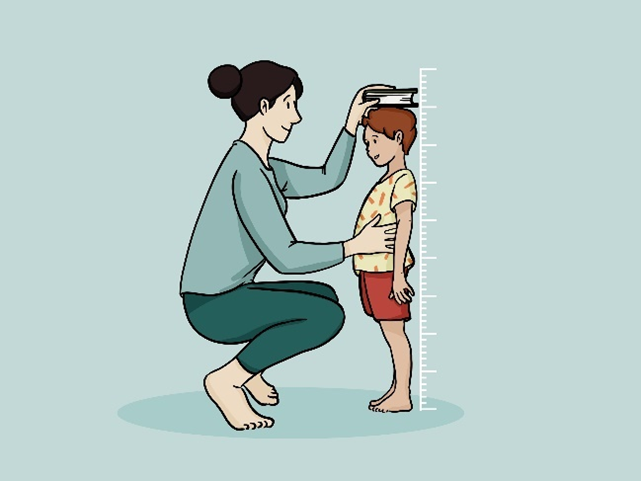
\includegraphics[scale=1.00]{img/Measurement.png}
    \caption{Pravidelné meranie výšky dieťaťa}
    \label{fig:measurement}
\end{figure}
\end{verbatim}

\begin{figure}[!ht]
    \centering
    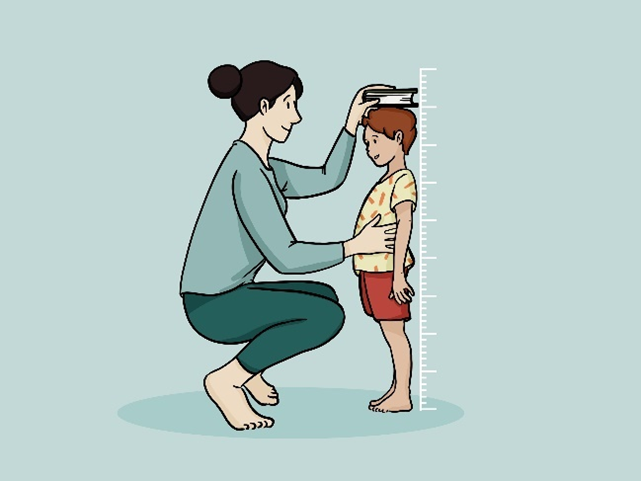
\includegraphics[scale=1.00]{img/Measurement.png}
    \caption{Pravidelné meranie výšky dieťaťa}
    \label{fig:measurement}
\end{figure}

\subsubsection{Umiestnenie obrázkov}\label{sec:figPlacement}
Na obrázok sa v~texte odkazujeme prostredníctvom čísla.
Môžeme písať o~tom, že na obrázku 1 vidíme to a~to
alebo použijeme skratku -- obr. 1.
Slovo obrázok aj skratku píšeme v~odkaze v~texte
malým začiatočným písmenom, ak sa nachádza vo vnútri vety.
Na každý obrázok v~práci by mal existovať odkaz v~texte.

Umiestnenie obrázku v rámci dokumentu riadi pomerne
komplikovaný algoritmus, čo nie vždy vedie k uspokojivým výsledkom.
Polohu plávajúceho objektu môžeme čiastočne ovplyvniť
nepovinným parametrom prostredia \verb|figure|.
V príklade, ktorý sme uviedli si môžeme všimnúť prítomnosť parametra \verb|h!| v hranatých zátvorkách
na konci prvého riadka.
Predstavuje požiadavku, že preferujeme,  aby sa obrázok nachádzal vo výslednom dokumente presne na tomto mieste. \LaTeX\ niekedy umiestni obrázok na začiatok nasledujúcej strany, prípadne aj inam.
Ak sa mu obrázok nepodarí umiestniť, zaradí ho až na
samý koniec kapitoly aj spolu so všetkými nasledujúcimi obrázkami.
To nebýva žiaduce a žiaľ, nemáme príliš veľa možností, ako takýto výsledok ovplyvniť.
Pomôže zmena rozmerov obrázku, prípadne jeho premiestnenie inam v zdrojovom kóde.
Odporúča sa, aby sa prostredie \verb|\begin{figure}...\end{figure}| nachádzalo mimo textového odseku, t. j. treba ho od okolitého textu oddeliť minimálne jedným prázdnym riadkom zhora aj zdola.

Na ovládanie umiestnenia plávajúceho objektu môžeme použiť tieto
parametre \verb|h|~(here) -- umiestnenie v mieste výskytu,
\verb|t|~(top) -- umiestnenie na stránke hore, \verb|b|~(bottom) --
umiestnenie na stránke dole, \verb|p|~(page) -- umiestnenie
na samostatnej stránke na konci kapitoly. Prvé tri
parametre môžu byť doplnené znakom výkričníka (\verb|!|),
ktorý požiadavku zosilňuje.
Jednotlivé parametre možno aj kombinovať.
Napríklad inštrukcia \verb|[!ht]| znamená, že chceme mať
obrázok na tom mieste, kde sa nachádza v zdrojovom kóde
a~ak to za žiadnu cenu nie je možné,
trebárs z~dôvodu nedostatku miesta pred koncom strany,
môže sa obrázok nachádzať aj v~hornej časti stránky.
Ani to však nemusí stačiť a~obrázok napokon nájdeme
na konci dokumentu.
V~takom prípade treba skúsiť niektoré
z~riešení spomenutých v~predchádzajúcom odseku.

\subsubsection{Označenie obrázku a text pod obrázkom}
Text pod obrázkom pozostáva z~označenia obrázku a z~vysvetľujúceho obsahu.
Mal by sa nachádzať spolu s~obrázkom na tej istej strane.

Text je dostatočne opisný,
aby bol jasný obsah obrázku aj pri rýchlom prechádzaní
práce bez nutnosti detailného čítania hlavného textu.
Ak opis pod obrázkom pozostáva iba z~jednej vety,
prípadne ide o~heslo bez vetnej štruktúry,
nepíšeme zaň bodku.
V~prípade viacerých viet už bodku alebo príslušné interpunkčné
znamienka použijeme na konci každej vety,
aj poslednej.
V príklade na obrázku \ref{fig:measurement} je text bez bodky
a~to je správne.

\subsubsection{Číslovanie a odkazy}
Obrázky číslujeme podľa výskytu v práci od čísla 1.
Používame jednoúrovňové číslovanie,
teda obrázok 1, obrázok 2, atď.
V~\LaTeX-u je automatické číslovanie obrázkov zabezpečené v definícii makra \verb|\caption|.

Odvolávanie sa na číslo obrázku rieši dvojica príkazov \verb|\label| a~\verb|\ref|.
Prvý príkaz zistí prítomnosť najbližšieho číselného
registra a priradí k nemu menovku, ktorú zadáme do argumentu.
Napríklad obrázok \ref{fig:measurement} má menovku \verb|fig:measurement|. Menovku volí autor textu, môže byť ľubovoľná, musí však začínať písmenom a nesmie obsahovať špeciálne znaky, ktoré majú v \TeX-u kategóriu vykonateľných príkazov (napr. \verb|\|, \verb|%|, \verb|#|, \verb|$|, zátvorky a podobne). Tiež treba venovať pozornosť tomu, aby sa rovnaká menovka nevyskytla v~texte v príkaze \verb|\label| viackrát, pretože by došlo k jej preťaženiu a znefunkčneniu odkazov.

Z praktických dôvodov sa ustálila prax začínať menovku skratkou typu číslovanej položky: \verb|fig| pre obrázok, \verb|eq| pri rovniciach, \verb|tab| ako menovka tabuľky, \verb|sec| v~prípade nadpisu, atď.

\subsection{Grafy}
Grafmi budeme nazývať zobrazenie vedeckých dát
najčastejšie vo forme dvojrozmerného grafu
závislosti dvoch alebo viacerých veličín.
Príklad takéhoto objektu je na obrázku \ref{fig:Graph1}.
Grafická reprezentácia vedeckých dát musí byť
v~prvom rade čitateľná, zreteľná a~jednoznačná.
Tomu treba prispôsobiť všetky zásady pri tvorbe grafov.

\begin{figure}[h!]
  \centering
  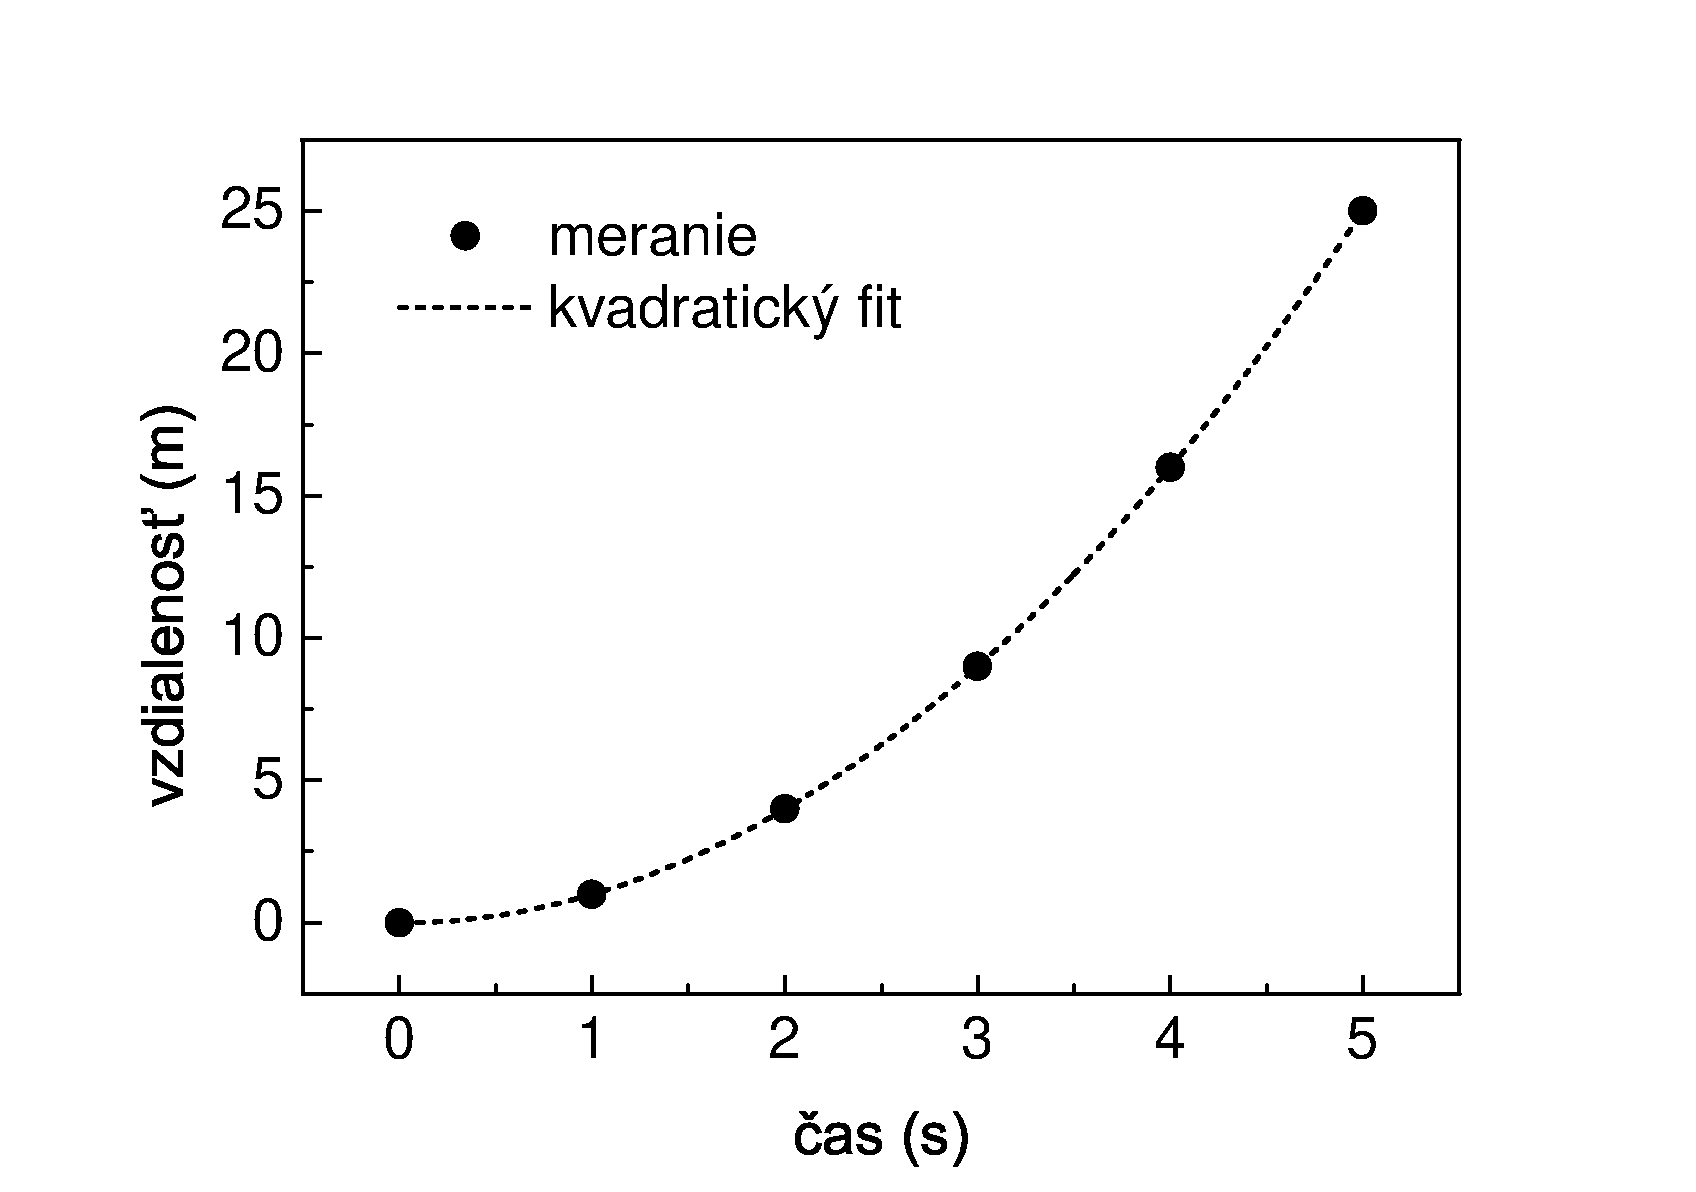
\includegraphics[scale=0.358]{img/Graph1}
  \caption{Ukážka grafu vytvoreného v externom programe a vloženého ako PDF súbor.
  Použité písmo je Arial s veľkosťou približne 10\,pt. Plné krúžky sú body merania a~prerušovaná čiara je kvadratický fit závislosti $s = at^2/2$, pričom $a = (2{,}00 \pm0{,}01)\,\mathrm{m\,s^{-2}}$.}
  \label{fig:Graph1}
\end{figure}

\subsubsection{Formát súboru}
Vektorové formáty SVG alebo PDF sú ideálna voľba pri exporte
z~grafických programov, napr. z~Excelu alebo Originu.
Ak takúto možnosť nemáme, treba grafy z externého softvéru
exportovať do bitmapového formátu, najlepšie PNG.
Stratový formát JPEG nie je na čiarovú grafiku vhodný.
Rozlíšenie bitmapového súboru by malo byť minimálne 600 dpi,
aby boli čiary ostré.
Znamená to, že ak predpokladáme veľkosť obrázku
$10\,\mathrm{cm} \times 7{,}5\,\mathrm{cm}$,
musí mať aspoň 2\,363\,px $\times$ 1\,772\,px (pixelov).

\subsubsection{Písmo a hrúbka čiar}
Písmo v grafe nemusí byť nevyhnutne Computer Modern.
V~obrázkoch a~schémach sa často používa
tzv. bezserifové alebo groteskové písmo ako napr. Arial,
ktoré je lepšie čitateľné.
Veľkosť písma v~obrázkoch by nemala byť menšia než
10\,pt,
čo je o~dva stupne menej ako základná veľkosť písma
v~dokumente.

Pozornosť treba venovať aj dostatočnej hrúbke čiar osí
a~grafického znázornenia dát,
aby boli viditeľné aj po vytlačení na bežnej tlačiarni.

\subsubsection{Prvky grafu}
Formálne prvky grafu sú osi s~dielikmi a~číslami,
názvy osí s~uvedením veličín, násobkov a~jednotiek,
mriežka a~legenda.
Medzi obsahové prvky zaraďujeme znázornené hodnoty vo forme
bodov alebo čiar.
Graf môže obsahovať aj názov grafu
a~doplňujúce texty,
prípadne ďalšie grafické prvky na zvýraznenie niektorých bodov,
oblastí a~podobne.

Bežný graf pozostáva zväčša z~dvoch navzájom kolmých číselných
osí – z~ľavej zvislej a~spodnej vodorovnej,
ktoré sa pretínajú v~ľavom dolnom rohu.
Na spodnej osi sa nachádzajú hodnoty nezávislej veličiny,
ľavá zvislá os obsahuje hodnoty závislej veličiny.
Rozsahy osí volíme tak,
aby korešpondovali s~intervalmi zobrazovaných hodnôt,
prípadne aby znázorňovali javy,
ktoré majú byť z grafu zrejmé.
Osi sa môžu pretínať aj v inom než nulovom bode.

\subsubsection{Označenie osí}
Osi musia byť riadne označené názvom alebo značkou veličiny,
jej jednotkou a~násobkom.
Nedodržanie tohto pravidla sa považuje za závažný nedostatok
a~autor musí mať na takýto krok obhájiteľný dôvod.
Jednotku spolu s~násobkom uzatvárame kvôli jednoznačnosti
do okrúhlych zátvoriek.
Hranaté zátvorky sa v knižnej tlači na tento účel nepoužívajú.

Os musí byť jasne rozdelená dielikmi,
ktoré sú kolmé na os a~predstavujú okrúhle hodnoty
zobrazovanej veličiny.
V blízkosti hlavných dielikov sa nachádzajú čísla prislúchajúce
hodnote dieliku.
Táto hodnota sa potom násobí s údajom v~zátvorke
v~opise osi a~spolu tvoria hodnoty zobrazenej fyzikálnej
veličiny aj s~jednotkou.

\subsubsection{Viacero grafov v jednom obrázku}
Priebehy dvoch a~viac nezávislých veličín môžeme nakresliť
do spoločných osí alebo použijeme pravú nezávislú zvislú os.
V~špeciálnych prípadoch môžeme využiť aj hornú vodorovnú os.
Ak chceme v~jednom obrázku zobraziť viacero grafov,
musí byť príslušnosť jednotlivých bodov a~čiar k~osiam jasná
z~legendy.
Legendu možno zahrnúť aj do textu pod obrázkom.

Graf znázorňujúci experimentálne hodnoty fyzikálnych veličín
zvykne byť uzavretý zhora aj sprava tak,
ako na obrázku \ref{fig:Graph1}.
Dve prekrížené otvorené osi sa používajú zväčša
v~prípade teoretického nákresu matematickej funkcie $y = f(x)$.

\subsection{Tabuľky}
Sumarizácia dát vo forme tabuliek prispieva
k~sprehľadneniu obsahu, zjednodušuje text
a~umožňuje autorovi zamerať sa pri formulácii myšlienok na
obsahovú stránku práce.
Tabuľka, podobne ako obrázok, patrí medzi plávajúce objekty
a preto nemusí byť umiestnená priamo na mieste v dokumente,
kde sa o nej zmieňuje text.
Zvyčajne ju umiestňujeme za odsek s~prvou zmienkou,
ale často býva aj súčasťou prílohy dokumentu,
najmä ak je rozsiahlejšia.

Zameriame sa teraz iba na tabuľky s~výsledkami meraní,
ktoré sa v~záverečných prácach vyskytujú najčastejšie.

Tabuľku označujeme slovom Tabuľka,
za ktorým nasleduje poradové číslo tabuľky podľa výskytu
v~texte.
Za číslom môže nasledovať dvojbodka a~text s~opisom obsahu
tabuľky.
V~prípade, že označenie neobsahuje opisný text,
dvojbodku vynecháme.
Opisný text nekončí bodkou,
ani iným interpunkčným znamienkom,
pokiaľ ide iba o názov alebo jednu oznamovaciu vetu.
Celý odsek s~označením, číslom a~opisom umiestňujeme
nad tabuľku (pozri napríklad tabuľku~\ref{tab:template}).

\begin{table}[h!]
  \caption{Vzorová tabuľka}
  \label{tab:template}
  \centering
  \begin{tabular}{@{}lrrrr@{}}
    \toprule
    \textbf{názov riadka} & \textbf{stĺpec 1} & \textbf{stĺpec 2} & \textbf{stĺpec 3} & \textbf{stĺpec 4} \\
    \midrule
    prvý riadok & hodnota 1 & hodnota 2 & hodnota 3 & hodnota 4\\
    druhý riadok & hodnota 5 & hodnota 6 & hodnota 7 & hodnota 8\\
    tretí riadok & hodnota 9 & hodnota 10 & hodnota 11 & hodnota 12\\
    \bottomrule
  \end{tabular}
\end{table}

Na tabuľky sa odvolávame pomocou ich čísla použitím dvojice makier
\verb|\label| a~\verb|\ref|.
Spôsob odkazovania je podobný ako v prípade obrázkov,
o~ktorom sme podrobne hovorili v časti \ref{sec:figPlacement}.

\subsubsection{Vzhľad tabuľky}
Jednoduchá tabuľka obsahuje hlavičku a~niekoľko
údajových riadkov.
Vzhľad tabuľky je otázka estetických preferencií autora.
Príliš veľa grafických prvkov znižuje obsahovú hodnotu a čitateľnosť tabuľky.
Formát, ktorý sme vybrali je inšpirovaný trendmi
v~knižnej sadzbe.
Tabuľka je zhora a~zdola ohraničená vodorovnými čiarami
\verb|\toprule| a~\verb|\bottomrule| z~knižnice \verb|booktabs|.
Podobne je čiarou \verb|\midrule| oddelená hlavička tabuľky
a~prípadne aj päta, ak ju použijeme.
Zvislé čiary sa používajú iba vo výnimočných prípadoch,
napríklad ak je tabuľka rozdelená na
dve evidentne oddelené časti.
Prípadne môžeme čiarou oddeliť prvý stĺpec s~opisom označenia riadka (tabuľka \ref{tab:LED}).
Jednotlivé riadky s~údajmi neoddeľujeme.
Tabuľka pôsobí harmonicky,
ak je text v~prvom stĺpci zarovnaný doľava
a~v~poslednom stĺpci doprava.

Prvý riadok môže byť vysádzaný polotučným
rezom (bold),
ak obsahuje tzv. hlavičku, teda názvy stĺpcov alebo názvy
a~jednotky veličín, ktorých hodnoty sú v~konkrétnom stĺpci.
Označenie veličín symbolom ($U$, $I$, $R$, $P$, a~pod.)
nepíšeme v~hlavičke tučným písmom,
aby sme dodržali pravidlo o~tom,
že veličiny by mali byť v~celom dokumente označené symbolom
rovnakého tvaru a typu.

\begin{table}[h!]
  \caption{Tabuľka parametrov štyroch diód LED.
  FWHM predstavuje šírku píku v~polovici intenzity
  spektrálneho maxima (\foreignlanguage{english}{\emph{Full-Width-Half-Maximum}}) pri vlnovej dĺžke~$\lambda_\mathrm m$.}
  \label{tab:LED}
  \centering
  \begin{tabular}{@{}l|rrrr@{}}
    \toprule
    dióda & $\lambda_\mathrm m\,(\mathrm{nm})$ & FWHM\,(nm) & žiarivý výkon\,$(10^{-5}\,\mathrm W)$ & farba \\
    \midrule
    LED 1 & $450 \pm 5$ & $20\pm2$ & $3\pm1$ & modrá\\
    LED 2 & $525 \pm 5$ & $25\pm3$ & $50\pm4$ & zelená\\
    LED 3 & $615 \pm 5$ & $15\pm1$ & $2\pm1$ & oranžová\\
    LED 4 & $630 \pm 5$ & $20\pm2$ & $5\pm1$ & červená\\
    \bottomrule
  \end{tabular}
\end{table}

\subsubsection{Obsah tabuľky}
Tabuľka s nameranými hodnotami obsahuje v~prvom riadku označenie
veličín a~to buď slovom alebo symbolom.
Za veličinou nasleduje jednotka v~okrúhlej zátvorke.
Hranaté zátvorky na tento účel nepoužívame.
Bezrozmerné relatívne veličiny uvádzame s~jednotkou (a. u.).
Ide o zaužívanú formu v~medzinárodnej vedeckej komunite na pomenovanie tzv. príslušnej jednotky (angl. \foreignlanguage{english}{arbitrary unit}).
Takto označujeme aj osi grafov rôznych relatívnych veličín.

Pred jednotkou môže byť označenie násobku
a~dielu a~to ako v~symbolickej forme (kA, nm, MW),
tak aj vo forme dekadického exponentu ($10^3$, $10^{-9}$, $10^6$).
Vyhýbame sa zápisom v~tvare 1E-3 alebo 10-3,
pretože sú mätúce.
Text hlavičky vlnová dĺžka ($10^{-7}$\,m) znamená,
že hodnoty v~celom stĺpci predstavujú veličinu vlnová dĺžka
a~sú uvedené v~jednotkách $10^{-7}$ metra.

Neistoty a~odchýlky zapisujeme k~hlavnej hodnote pomocou
znaku $\pm$ alebo do zvláštneho stĺpca,
ktorý príslušne označíme.
Ďalšie spôsoby zápisu neistôt uvádza príslušná norma (napr. STN 01 6910: 2022 \cite{stn016910}).

%%%%%%%%%%%%%%%%%%%%%%%%%%%%%%%%%%%%%%%
%%                                   %%
%% Výpisy kódov programu a algoritmy %%
%%                                   %%
%%%%%%%%%%%%%%%%%%%%%%%%%%%%%%%%%%%%%%%
\subsection{Výpisy kódov programu a algoritmy}
\label{sec:listings}
Ak je súčasť cieľov práce tvorba softvéru, prípadne analýza programátorských riešení,
je žiaduce uvádzať časti kódov vo forme krátkych výpisov (angl. \foreignlanguage{english}{\emph{listing}}).
Existuje niekoľko balíčkov, ktoré umožňujú zahrnúť časti kódov do textu práce.
Šablóna \verb|FEIstyle| používa balík \verb|listings|.
Prostredie \verb|lstlisting| vytvorí blok kódu s~menovkou Výpis kódu s~číslom výpisu.
Makro \verb|\FEIlistOfListings| na začiatku dokumentu vygeneruje zoznam všetkých výpisov,
ktorý nie je povinnou súčasťou práce,
býva však dobrým zvykom uvádzať ho najmä v~informatických študijných programoch.

Ukážka kódu je vo výpise~\ref{lst:main-c}.
V dodatku \ref{att:listings} nájdeme príklad výpisu obsahu externého textového súboru.
Ďalšie podrobnosti možno nájsť v~dokumentácii k~balíčkom%
\footnote{\href{https://ctan.org/pkg/listings}{\texttt{ctan.org/pkg/listings}}}
alebo v~tutoriáli služby Overleaf%
\footnote{\texttt{\href{https://www.overleaf.com/learn/latex/Code_listing}{www.overleaf.com/learn/latex/Code\_listing}}}.

\begin{lstlisting}[,
  caption={Ukážka výpisu kódu programu},
  label={lst:main-c},
  language=c,
  style=code-listing
]
/* Hello World program */

#include<stdio.h>

struct cpu_info {
    long unsigned utime, ntime, stime, itime;
    long unsigned iowtime, irqtime, sirqtime;
};

main()
{
    printf("Hello World");
}
\end{lstlisting}

\subsection*{Algoritmy}
Dvojica balíkov%
\footnote{\href{https://ctan.org/pkg/algorithms}{\texttt{ctan.org/pkg/algorithms}}}
\verb|algorithm|
a~\verb|algorithmic| uľahčuje zápis algoritmizácie pomocou tzv. pseudokódov.
Tieto nástroje sa uplatňujú najmä v prípade teoretických prác v~oblasti informatiky a~softvérového inžinierstva.
Šablóna FEIstyle načíta balíky automaticky a~tiež definuje makro \verb|\FEIlistOfAlgorithms|, ktoré na začiatku vytvorí zoznam všetkých algoritmov, v~záverečnej práci.
Príkaz možno vynechať alebo označiť riadok ako poznámku znakom \verb|%|, zoznam sa tak nevytvorí. Ako príklad uvádzame algoritmus \ref{alg:calculation-1} v~dodatku \ref{att:algorithms}.

Ďalšie podrobnosti získame z~tutoriálov%
\footnote{\href{https://www.overleaf.com/learn/latex/Algorithms}{\texttt{www.overleaf.com/learn/latex/Algorithms}}}
alebo z~dokumentácie k~jednotlivým balíčkom.

%%%%%%%%%%%%%%%%%%%%%%%%%%%%%%%%%
%%                             %%
%% Citovanie externých zdrojov %%
%%                             %%
%%%%%%%%%%%%%%%%%%%%%%%%%%%%%%%%%
\section{Citovanie externých zdrojov}\label{sec:citation}
V~súvislosti s~preberaním časti obsahu iných diel
rozoznávame dva pojmy. Sú to citát a~citácia.

Citát je doslovná reprodukcia prevzatého textu,
ktorý môžeme v~práci použiť dvomi spôsobmi.
Buď ako súčasť odseku textu,
alebo celý citovaný text vysádžeme v~samostatnom odseku.
V oboch prípadoch je zvykom citovaný text uzavrieť do úvodzoviek
a~zvýrazniť šikmým rezom písma.
Za citovaným textom uvedieme meno autora,
prípadne názov diela, rok a nasleduje číslo bibliografického
zdroja v~hranatých zátvorkách uvádzajúce poradie
v~zozname použitej literatúry v~závere práce.

Na citovanie v rámci odseku môžeme využiť makrá \verb|\uv| pre
správne slovenské úvodzovky a \verb|\emph|,
ktoré zabezpečí vytlačenie textu kurzívou.

Samostatne vysádzaný citát uzavrieme v \LaTeX-u do prostredia
\verb|\begin{quote}...| \verb|\end{quote}|.

Citácia je nepriamo prebraná a~prerozprávaná
časť citovanej práce.
Môže to byť vedecká myšlienka, odkaz na výsledky výskumu,
dôležitý poznatok, matematický vzťah a~podobne.
Schopnosť študenta pracovať s~literatúrou a~s~externými zdrojmi
je dôležitý moment pri hodnotení spôsobilosti uchádzača
o~vysokoškolský titul.
Tomuto aspektu práce treba preto venovať patričnú pozornosť.

Užitočný prehľad spôsobov citácií ponúkajú autorky
Beáta Bellérová a~Lucia Lichnerová v~článku v~časopise ITLib~\cite{Lichnerova2023Nove}.

\subsection{Odkazy na citované diela}
Vo vedecko-technických oblastiach, do ktorých patria aj študijné programy na našej fakulte, je zvykom používať numerický systém citovania. Jednotlivé zdroje sú očíslované podľa poradia výskytu v texte, pričom číslo zdroja uvádzame v hranatých zátvorkách.
Citovanie sa riadi technickou normou STN ISO 690: 2022 Informácie a dokumentácia: Návod na tvorbu bibliografických odkazov na informačné pramene a~ich citovanie~\cite{iso690}.

Systém \LaTeX\ umožňuje pracovať s citáciami niekoľkými spôsobmi.
Šablóna FEIstyle pracuje s balíčkom \verb|biblatex| na správu citácií. Jeho základom je externý databázový súbor \texttt{bibliography.bib},
ktorý sa nachádza v hlavnom priečinku projektu záverečnej práce.
Súbor obsahuje bibliografické záznamy citovaných diel
v špecifickom formáte.
Každý záznam začína jedinečným identifikátorom, ktorý zvyčajne
volíme tak, aby sme si ho jednoducho pamätali.
Ak totiž v texte chceme dielo citovať, napíšeme makro \verb|\cite{identifikator}| a~v~práci sa automaticky objaví poradové číslo citovaného diela v hranatej zátvorke.
Číslo citácii pridelí externý program \textsl{biber},
ktorý prejde celý dokument, identifikuje výskyty makra \verb|\cite|, zoradí citované diela podľa výskytu v~práci,
pridelí im čísla a vytvorí podklady na zoznam literatúry na konci práce.
Pri ďalšom spustení kompilátora \TeX-u dôjde k~nahradeniu makier
\verb|\cite| číslami v hranatých zátvorkách a makro šablóny
\verb|\FEIbibliography| vytvorí zoznam literatúry s nadpisom
prvej úrovne Literatúra.

Pri použití bibliografie odporúčame použiť dávkový súbor
\texttt{Makefile} alebo spustiť externý program \texttt{biber}
po prvej kompilácii a~potom skompilovať dokument ešte dvakrát.
Posledná kompilácia zabezpečí správne čísla strán v obsahu.
Online nástroj Overleaf robí všetky potrebné kroky v jednom behu,
kompiláciu tu stačí spustiť iba raz.

\subsection{Bibliografické záznamy}
V zozname použitej literatúry v~závere práce sa nachádzajú
podrobné záznamy použitých zdrojov.
Sú to najmä mená autorov, názov článku alebo číslo kapitoly
knihy, názov časopisu alebo knihy, vydavateľ, rok vydania,
strana, na ktorej sa nachádza citovaný článok a podobne.
V~prípade webových stránok je potrebné uviesť internetovú adresu
a~dátum, kedy sme informáciu zo stánky čerpali.
Dôležité je, aby boli informácie na základe týchto detailov
ľahko a jednoznačne dohľadateľné.
Norma STN ISO 690: 2022 tiež definuje formu takéhoto zoznamu~\cite{iso690}.

V~tejto publikácii formátujeme použitú literatúru
podľa štýlu iso-numeric \cite{Hoftich2022iso690} balíka \texttt{biblatex},
\footnote{\href{https://ctan.org/pkg/biblatex}{\texttt{ctan.org/pkg/biblatex}}}
ktorý do veľkej miery rešpektuje doteraz zaužívané zvyklosti
a~je navrhnutý tak,
aby spĺňal odporúčania normy aj v~slovenskom jazyku.

\subsubsection{Príklad záznamu v databázovom súbore .bib}\label{sec:citExample}
Súbor \texttt{bibliography.bib} je textový súbor, ktorý musí mať predpísanú štruktúru.
Môžeme ho vytvoriť ručne alebo použiť niektorý zo systémov na správu publikácií a~citácií ako sú JabRef, Mendeley, Zotero a podobne.

Nasledujúci bibliografický záznam
\begin{trivlist}
  \item STEINEROVÁ, J. Princípy formovania vzdelania
  v~informačnej vede. \textit{Pedagogická revue.} 2000, \textbf{2}(3), 8--16.
\end{trivlist}
vyzerá v zdrojovom súbore \texttt{bibliography.bib} takto:
\begin{verbatim}
@article{Steinerova2000Principy,
  author  = {J. Steinerová},
  journal = {Pedagogická revue},
  title   = {Princípy formovania vzdelania v informačnej vede},
  year    = {2000},
  number  = {3},
  pages   = {8--16},
  volume  = {2},
}
\end{verbatim}

Každý záznam začína symbolom \verb|@| a nasleduje typ publikácie definovaných v dokumentácii k balíčku Bib\LaTeX.
Okrem článku (\verb|article|) to môže byť aj kniha (\verb|book|),
príspevok v zborníku konferencie (\verb|inproceedings|),
webová stránka (\verb|online|),
správa (\verb|techreport|),
všeobecný záznam (\verb|misc|) a mnohé iné.

Prvý povinný údaj je jedinečný identifikátor, ktorý je ľubovoľný.
Odporúča sa však aby obsahoval priezvisko prvého autora, rok vydania a prvé slovo názvu.

Jednotlivé položky databázového záznamu sú oddelené čiarkou,
za posledným poľom už čiarka nie je.

Každý typ záznamu má iné požiadavky na polia.
Niektoré základné vlastnosti opíšeme v nasledujúcom texte.
Viac informácií možno získať v príslušnej dokumentácii~\cite{Hoftich2022iso690}.

\subsubsection{Prvky bibliografického záznamu}
Zoznam použitej literatúry obsahuje informácie o jednotlivých zdrojoch. Je potrebné mať na pamäti, aby záznamy boli jasné, stručné a jednoznačne identifikovateľné. Bežne zorientovaný čitateľ práce, ktorý sa pohybuje v okruhu tém práce by mal byť schopný identifikovať jednotlivé diela na prvé pozretie. Prípadný záujemca o detailné štúdium problematiky by si mal vedieť na základe záznamu vyhľadať citovanú publikáciu buď na internete alebo v knižnici. Týmito pravidlami sa riadime pri vytváraní zoznamu použitej literatúry.

Uvedieme niekoľko jednoduchých a~najčastejších príkladov bežného
spôsobu citovania.
Snaha je, aby sme sa prirodzene naučili formy uvádzania
bibliografických záznamov v~našej oblasti vedy a techniky
a~dokázali vytvoriť správnu databázu zdrojov v systéme Bib\LaTeX.

\subsubsection*{Mená tvorcov}
V zozname literatúry majú formu: PRIEZVISKO, Meno alebo PRIEZVISKO, M. a~navzájom sú oddelené bodkočiarkou.
Za zoznamom autorov nasleduje bodka.

\subsubsection*{\normalsize Pole v .bib súbore}
\begin{verbatim}
author = {Meno1 Priezvisko1 and Meno2 Priezvisko2 and Meno3 Prizvisko3}
\end{verbatim}
Autorov zapisujeme ako \verb|Meno Priezvisko| a~oddeľujeme ich kľúčovým slovom and.
Môžeme tiež použiť obrátený tvar \verb|Priezvisko, Meno and|\dots s~čiarkou medzi priezviskom a~menom.

\subsubsection*{Názov}
Názov článku píšeme normálnym písmom.
Názov nosného informačného zdroja (kniha, časopis, zborník) píšeme kurzívou.

\subsubsection*{\normalsize Polia v .bib súbore}
\begin{verbatim}
title = {}
booktitle = {}
\end{verbatim}

\subsubsection*{Dátum}
Pri každej publikácii musí byť uvedený aspoň rok vydania
vo formáte YYYY, t. j. 2024.
V prípade online zdrojov treba uvádzať aj presný dátum,
kedy sme zdroj použili.
Vkladáme ho do hranatých zátvoriek s~kľúčovým slovom cit.
Odporúčame použiť formát [cit. YYYY-MM-DD].
Ak sme teda informáciu z webovej stránky získali dňa
14. mája 2023,
napíšeme to takto: [cit. 2023-05-14].
Ide o medzinárodne akceptovaný a~zrozumiteľný tvar zápisu dátumu.

\subsubsection*{\normalsize Polia v .bib súbore}
\begin{verbatim}
year = {2024}
date = {2024-12-31}
\end{verbatim}

\subsubsection*{Dostupnosť}
Myslí sa tým dostupnosť na internete najmä prostredníctvom webu.
Uvádzame buď úplnú webovú adresu alebo DOI číslo.
Nepíšeme oba údaje, preferujeme DOI.
Tento údaj sa nachádza zväčša na konci záznamu za kľúčovým výrazom Dostupné na.

\subsubsection*{\normalsize Polia v .bib súbore}
\begin{verbatim}
url = {}
doi = {}
eprint = {}
\end{verbatim}
Ak uvedieme viacero polí, Bib\LaTeX\ zväčša vyberie iba jedno
podľa preferencií špecifikovaných v~definičnom súbore.

\subsubsection*{Ročník alebo zväzok a číslo časopisu}
Vedecké periodiká vychádzajú v tzv. zväzkoch (angl. \foreignlanguage{english}{\it volume}).
Zväzky sa môžu deliť na čísla
(angl. \foreignlanguage{english}{\it issue} alebo
\foreignlanguage{english}{\it number}).
Zväzok a číslo zapisujeme buď pomocou skratiek vol. a~iss.
(prípadne no. podľa skutočného členenia jednotlivých vydaní konkrétneho časopisu),
alebo preferujeme zaužívanú skrátenú formu,
pri ktorej nepoužijeme slovné skratky,
ale píšeme len čísla,
pričom zväzok vytlačíme tučným rezom (bold)
tesne nasledovaný číslom časopisu normálnym písmom
v~okrúhlych zátvorkách.
Napríklad zväzok 15, číslo 8 môžeme zapísať
ako vol. 15, iss. 8 alebo \textbf{15}(8).

\subsubsection*{\normalsize Polia v .bib súbore}
\begin{verbatim}
volume = {}
number = {}
\end{verbatim}

\subsection{Článok v odbornom periodiku}
Záznam musí obsahovať mená autorov (tvorcov), názov článku, názov časopisu, dátum alebo iba rok vydania, ročník alebo zväzok (volume) a číslo vo zväzku (issue), číslo prvej strany, prípadne rozsah strán, na ktorých sa nachádza.

\subsubsection*{\normalsize Nepovinné údaje}
Ak je článok dostupný online, je dobré, ak sa v zápise objaví aj webová adresa digitálnej verzie článku. Vedecké publikácie majú pridelený jedinečný kód, tzv. DOI (Digital Object Identifier – identifikátor digitálneho objektu), ktorý tiež môže byť súčasťou bibliografického zápisu. Ďalšou nepovinnou časťou je International Standard Serial Number (ISSN), teda medzinárodné štandardné sériové číslo, ktoré sa prideľuje časopisom.

\subsubsection*{\normalsize Printový časopis}
\begin{trivlist}
\item TVORCOVIA. Názov článku. \textit{Názov periodika.} Rok vydania, \textbf{zväzok}(časť), rozsah strán. Dostupnosť.
\end{trivlist}

\subsubsection*{\normalsize Online časopis}
\begin{trivlist}
\item TVORCOVIA. Názov článku. \textit{Názov periodika} [online]. Rok vydania, \textbf{zväzok}(časť), rozsah strán (ak je k dispozícii). [cit. yyyy-mm-dd]. Dostupnosť.
\end{trivlist}

\subsubsection*{\normalsize Príklady}
Prvý príklad je z~časti
\ref{sec:citExample} odkazuje na článok s názvom Princípy formovania vzdelania v informačnej vede od autorky Jely Steinerovej, ktorý vyšiel v roku 2000 v 3. čísle 2. ročníka časopisu Pedagogická revue. Článok sa v časopise nachádza na stranách 8 až 16.

V druhom príklade skratka et. al. (skratka latinského slovného spojenia \textit{et alii}, vo význame a~iní) za menom autora znamená, že článok má viacero autorov (bežne viac než 5) a nemusíme ich všetkých uvádzať.
V slovenských textoch sa môže použiť skratka a~kol. (a~kolektív).

Tretí príklad je príklad online časopisu, ktorý možno nájsť na internete. Príznak [online] a~dátum citovania [cit. 2023-01-10] sa objaví v zozname literatúry, keď v súbore \verb|bibliography.bib| použijeme pole \verb|urldate|.

\begin{enumerate}
\item STEINEROVÁ, J. Princípy formovania vzdelania v informačnej vede. \textit{Pedagogická revue}. 2000, \textbf{2}(3), 8–16.
\item BEŇAČKA, J. et al. A better cosine approximate solution to pendulum equation. \textit{International Journal of Mathematical Education in Science and Technology}, 2009, \textbf{40}(2), 206–215.
\item HOGGAN, D. B. Challenges, Strategies, and Tools for Research Scientists. Electronic Journal of \textit{Academic and Special Librarianship} [online]. 2009, \textbf{3}(3). [cit. 2023-01-10]. Dostupné z: \texttt{http://southernlibrarianship.icaap.org/content/ v03n03/Hoggan\_d01.htm}. ISSN 1525-321X.
\end{enumerate}

\subsubsection*{\normalsize Zápis v zdrojovom .bib súbore}
\begin{verbatim}
@article{Steinerova2000Principy,
  author  = {J. Steinerová},
  journal = {Pedagogická revue},
  title   = {Princípy formovania vzdelania v informačnej vede},
  year    = {2000},
  number  = {3},
  pages   = {8--16},
  volume  = {2},
}

@article{Benacka2009Abetter,
  author  = {Ján Benačka and others},
  title   = {A better cosine approximate solution to pendulum
             equation},
  journal = {International Journal of Mathematical Education in Science
             and Technology},
  volume  = {40},
  number  = {2},
  pages   = {307--308},
  year    = {2009},
  doi     = {10.1080/00207390802419594},
}

@article{Hoggan2002Challenges,
  author  = {Danielle Bodrero Hoggan},
  journal = {Electronic Journal of Academic and Special Librarianship},
  title   = {Challenges, Strategies, and Tools for Research Scientists:
             Using Web-Based Information Resources},
  year    = {2002},
  number  = {3},
  volume  = {3},
  url     = {https://southernlibrarianship.icaap.org/content/v03n03/
             Hoggan_d01.htm},
  urldate = {2023-01-10},
}
\end{verbatim}

\subsection{Monografia a~kniha}
\begin{trivlist}
\item TVORCOVIA. Názov knihy. Vydanie. Mesto: Vydavateľ, Rok vydania. ISBN.
\end{trivlist}

\subsubsection*{\normalsize Príklady}
\begin{enumerate}
\item OBERT, V. \textit{Návraty a odkazy}. Nitra: Univerzita Konštantína Filozofa, 2006. ISBN 80-8094-046-0.

\item TIMKO, J.; SIEKEL, P.; TURŇA, J. Geneticky modifikované organizmy. Bratislava: Veda, 2004. ISBN 80-224-0834-4.
\end{enumerate}

\subsubsection*{\normalsize Zápis v zdrojovom .bib súbore}
\begin{verbatim}
@book{Obert2006Navraty,
  author    = {Viliam Obert},
  publisher = {Univerzita Konštantína Filozofa},
  title     = {Návraty a odkazy},
  year      = {2006},
  address   = {Nitra},
  isbn      = {80-8094-046-0},
}

@book{Timko2004Geneticky,
  author    = {Jozef Timko and Peter Siekel and Ján Turňa},
  publisher = {Veda},
  title     = {Geneticky modifikované organizmy},
  year      = {2004},
  isbn      = {80-224-0834-4},
}
\end{verbatim}

\subsection{Záverečná a~vedecko-kvalifikačná práca, správa}
AUTOR. \textit{Názov práce}. Mesto, Rok vypracovania. Typ práce. Inštitúcia

\subsubsection*{\normalsize Príklady}
\begin{enumerate}
  \item MIKULÁŠIKOVÁ, M. \textit{Didaktické pomôcky pre praktickú výučbu na hodinách výtvarnej výchovy pre 2. stupeň základných škôl.} Nitra, 1999. Diplomová práca. Univerzita Konštantína Filozofa

  \item BAUMGARTNER, J. et al. \textit{Ochrana a udržiavanie genofondu zvierat, šľachtenie zvierat.} Nitra, 1998. Výskumná správa. VÚŽV.
\end{enumerate}

\subsubsection*{\normalsize Zápis v zdrojovom .bib súbore}
\begin{verbatim}
@thesis{Mikulasikova1999Didakticke,
  author  = {M. Mikulášiková},
  title   = {Didaktické pomôcky pre praktickú výučbu na hodinách
             výtvarnej výchovy pre 2. stupeň základných škôl},
  address = {Nitra},
  year    = {1999},
  type    = {Diplomová práca},
  school  = {Univerzita Konštantína Filozofa},
}

@report{Baumgarntner1998Ochrana,
  author      = {J. Baumgartner and others},
  institution = {VÚŽV},
  title       = {Ochrana a udržiavanie genofondu zvierat, šľachtenie
                 zvierat},
  address     = {Nitra},
  year        = {1998},
  type        = {Výskumná správa},
}
\end{verbatim}

\subsection{Príspevok v zborníku konferencie, časť knihy}
Ak citujeme iba jednu kapitolu knihy,
prípadne ide o~príspevok z~neperiodického zborníka,
uvedieme za názvom príspevku (kapitoly)
kľúčové slovo In:, po dvojbodke nasleduje zoznam editorov zborníka a názov zborníka alebo knihy:
\begin{trivlist}
  \item TVORCOVIA. Názov príspevku. In: EDITORI (ed.). \textit{Názov zborníka.} Mesto: Vydavateľ, Rok vydania, zväzok, s. rozsah strán, zv. číslo. ISBN. ISSN. Dostupnosť.
\end{trivlist}

\subsubsection*{\normalsize Príklady}
\begin{enumerate}
  \item ZEMÁNEK, P. The machines for ``green works'' in vineyards and their economical evaluation. In: \textit{9th International Conference: proceedings. Vol. 2. Fruit Growing and viticulture.} Lednice: Mendel University of Agriculture a Forestry, 2001, zv. 2, s. 262–268. ISBN 80-7157-524-0.

  \item CHLPÍK, J.; KURTULÍK, M.; KOTOROVÁ, S.; CIRÁK, J. Spectroscopic ellipsometry of Au nanoparticles layers. In: SITEK, J.; VAJDA, J.; JAMNICKÝ, I. (ed.). \textit{AIP Conference Proceedings.} 2024, zv. 3054, s. 080004. Č. 1. ISSN 0094-243X. Dostupné z doi: 10.1063/5.0187526.
\end{enumerate}

\subsubsection*{\normalsize Zápis v zdrojovom .bib súbore}
\begin{verbatim}
@InProceedings{Zemanek2001TheMachines,
  author    = {P. Zemánek},
  booktitle = {9th International Conference: proceedings. Vol. 2. Fruit
               Growing and viticulture},
  title     = {The machines for ``green works'' in vineyards and their
               economical evaluation},
  volume    = {2},
  year      = {2001},
  pages     = {262--268},
  publisher = {Mendel University of Agriculture and Forestry},
  address   = {Lednice},
  isbn      = {80-7157- 524-0},
}

@InProceedings{ChlpikSpectroscopic2024,
  author    = {Chlpík, Juraj and Kurtulík, Matej and Kotorová, Soňa
               and Cirák, Július},
  date      = {2024-01},
  title     = {Spectroscopic ellipsometry of Au nanoparticles
               layers},
  editor    = {Jozef Sitek and Ján Vajda and Igor Jamnický},
  doi       = {10.1063/5.0187526},
  number    = {1},
  pages     = {080004},
  volume    = {3054},
  issn      = {0094-243X},
  booktitle = {AIP Conference Proceedings},
}
\end{verbatim}

\subsection{Webová stránka, sociálna sieť, video}
Pri multimediálnom online obsahu často nepoznáme autora,
prípadne je komplikované zistiť názov webovej stránky.
Snažíme sa teda zahrnúť čo najviac jednoznačných informácií,
najmä webovú adresu, dátum publikovania a dátum citovania.
\begin{trivlist}
  \item TVORCOVIA. \textit{Názov obsahu} [online]. Platforma, dátum publikovania [cit. dátum citovania]. Dostupnosť.
\end{trivlist}

\subsubsection*{\normalsize Príklady}
\begin{enumerate}
  \item VALKO, P. \textit{M31, M32 a jeden Starlink k tomu} [online]. Facebook, 2024-08-30 [cit. 2024-09-06]. Dostupné z: \texttt{https://www.facebook.com/share/p/S93xZoz9Rbnh
  dQ7M}.

  \item \textit{Why lenses can't make perfect images} [online]. Youtube, 2017-10-18 [cit. 2024-08-25]. Dostupné z: \texttt{https://youtu.be/DDoryfCXxPI?si=hC5Kuuf4p3OxOOsm}.
\end{enumerate}

\subsubsection*{\normalsize Zápis v zdrojovom .bib súbore}
\begin{verbatim}
@online{Valko2024M31,
  author       = {Pavol Valko},
  title        = {31, M32 a jeden Starlink k tomu},
  howpublished = {online},
  date         = {2025-08-30T00:03:00},
  url          = {https://www.facebook.com/share/p/S93xZoz9RbnhdQ7M},
  urldate      = {2024-09-06},
  publisher    = {Facebook},
}

@online{WhyLenses2017,
  title        = {Why lenses can’t make perfect images},
  howpublished = {online},
  date         = {2025-10-18},
  url          = {https://youtu.be/DDoryfCXxPI?si=hC5Kuuf4p3OxOOsm},
  urldate      = {2024-08-25},
  publisher    = {Youtube},
}
\end{verbatim}

\subsection{Ako citovať technické normy}
K normám nemusíme uvádzať autorov, ak ide o slovenskú normu STN, netreba ani vydavateľa. Dôležité je číslo normy a rok vydania.

\begin{trivlist}
\item \textit{Číslo normy. Názov: Podnázov.} Mesto: Vydavateľ. Rok vydania.
\end{trivlist}

\subsubsection*{\normalsize Príklad}
\begin{itemize}
  \item \textit{STN ISO 690: 2023. Informácie a~dokumentácia: Návod na tvorbu bibliografických odkazov na informačné pramene a ich citovanie.} Bratislava: Slovenský ústav technickej normalizácie, 2023.
\end{itemize}

\subsubsection*{\normalsize Zápis v zdrojovom .bib súbore}
\begin{verbatim}
@report{iso690,
  title     = {STN ISO 690: 2022. Informácie a~dokumentácia},
  subtitle  = {Návod na tvorbu bibliografických odkazov na informačné
               pramene a~ich citovanie},
  address   = {Bratislava},
  publisher = {Slovenský ústav technickej normalizácie},
  year      = {2022},
}
\end{verbatim}

% LocalWords:  zostručnenie Bib vý nok výk le ok ax bx ds dt dx Eq CoulombVec
% LocalWords:  eq px lrrrr FWHM Full Width rrrr kA Technology HOGGAN Challenges
% LocalWords:  Strategies Tools Research Scientists Electronic Academic Special
% LocalWords:  Librarianship Hoggan OBERT TIMKO SIEKEL MIKULÁŠIKOVÁ BAUMGARTNER
% LocalWords:  VÚŽV ed ZEMÁNEK machines green works vineyards their economical
% LocalWords:  evaluation th Conference proceedings Fruit Growing viticulture
% LocalWords:  Mendel University Agriculture Forestry CHLPÍK KURTULÍK KOTOROVÁ
% LocalWords:  CIRÁK Spectroscopic ellipsometry nanoparticles layers SITEK doi
% LocalWords:  JAMNICKÝ VALKO Starlink Facebook dQ Why lenses can perfect
% LocalWords:  images Youtube
